\documentclass[12pt,toc=bibnumbered, a4paper,twoside]{scrreprt}

\usepackage{epsfig}
\usepackage{subfigure}
\usepackage{calc}
\usepackage{amssymb}
\usepackage{amstext}
\usepackage{amsmath}
\usepackage{amsthm}
\usepackage{multicol}
\usepackage{pslatex}
\usepackage{natbib}
\usepackage{booktabs}
\usepackage{tabularx}
\usepackage{algorithm}
\usepackage{mdwlist}
\usepackage{url}
\usepackage[noend]{algpseudocode}
\usepackage[small]{caption}
\usepackage{setspace}

\DeclareMathOperator*{\argmax}{arg\,max}
\DeclareMathOperator*{\argmin}{arg\,min}
\newcommand{\figref}[1]{Figure~\ref{#1}}
\renewcommand{\eqref}[1]{Equation~(\ref{#1})}
\algrenewcommand{\algorithmicrequire}{\textbf{Input:}}
\algrenewcommand{\algorithmicensure}{\textbf{Output:}}


\renewcommand*{\thefootnote}{\fnsymbol{footnote}}
\newcommand{\W}{\mathcal{W}}

\newcommand{\given}{\, | \,}
\newcommand{\B}[1]{\textbf{#1}}

\begin{document}

%\title{Learning a Loopy Model For Semantic Segmentation Exactly}


\begin{titlepage}
\begin{center}
\vspace*{1in}
\textbf{{\LARGE PhD Thesis}}
\par
\vspace{1.5in} {\large Andreas Mueller}
 \par \vfill A Thesis submitted for the degree of Doctor of Philosophy
\par \vspace{0.5in}
Department IV, Institute for Computer Science
\par \vspace{0.5in}
Friedrich-Willhelm Universitaet Bonn \par
\vspace{0.5in} September 2013 \end{center}

\end{titlepage}

\pagenumbering{Roman}

\tableofcontents

%\listoffigures
%\listoftables
\chapter*{Acknowledgements}

\begin{abstract} abstract
\end{abstract}

\pagenumbering{arabic}


\chapter{Information Theoretic Clustering for Object Class Discovey}
\chapter{Information Theoretic Clustering}\label{ch:itm}

Before we start our investigation of semantic segmentation and object class segmentation,
we look into a general purpose clustering algorithm.
%
In clustering, the goal is to divide data points into homogeneous subsets, called
clusters.
Many different formulations of the clustering problem are given in the literature.
%
In the context of this work, clustering plays an important role in many respects:
\begin{itemize}
    \item Clustering, as a purely unsupervised method, is on one end of the
        spectrum of algorithms we investigate.  When using per-image or
        per-pixel supervision as in the later chapters, we can use clustering
        to calibrate our expectation of what semi-supervised and supervised
        algorithms should be able to achieve.

    \item Clustering algorithms build the basis of most superpixel algorithms, and
        better clustering algorithms can lead to better superpixel algorithms.

    \item As many other computer vision algorithms, our segmentation methods
        depends on bag-of-feature representations of segments or images. These
        are built using a vocabulary of visual words that is usually created
        via clustering.
\end{itemize}

So not only is clustering one of the fundamental problems in machine learning, it is also
an important building block for other methods in this work.
%
Most algorithms are based on ad-hoc criteria such as intra-cluster similarity
and inter-cluster dissimilarity.
An alternative approach is to formalize clustering using an information
theoretic framework, where one considers inputs as well as cluster assignments
as random variables.  The goal is then to find an assignment of data points to
clusters that maximizes the mutual information between the assignments and the
observations.

In the following, we rely on a non-parametric estimator of the data entropy to find 
clusterings of maximum mutual information.
%
The use of non-parametric estimates allows a data-driven approach, without 
making strong assumptions on the form of the data distribution.
%
As a consequence, we obtain a very flexible model that, for example, allows 
non-convex clusters.
%
The resulting objective is easy to evaluate, but difficult to optimize
over. We overcome this by proposing an efficient approximate optimization
based on Euclidean minimum spanning trees.
%
Because the estimator and the optimization are both parameter-free, 
the only free parameter of the algorithm is the number of clusters, 
which makes it very easy to use in practice.
%
The non-parametric entropy estimate we
are using is applicable only if the data distribution is absolute continuous and
therefore can not be applied if the data lies on a proper submanifold.
We show how to overcome this obstacle in practice by using an estimate of the
intrinsic dimensionality of the data.
%
The contributions of this chapter are:
\begin{itemize}
    \item Proposing the use of a MST-based entropy estimator in information theoretic clustering.
    \item Giving a fast algorithm for a relaxed version of the resulting problem.
    \item Showing the practicality on a number of synthetic and real datasets.
    \item Extending the clustering to data on submanifolds by estimating intrinsic dimensionality.
\end{itemize}

%CHL: Maybe use this somewhere else, here it sounds redundant.
%While other algorithms have to rely on continuous, gradient-based techniques,
%we can rely on fast, combinatorial optimization.
%
%The run time of the proposed algorithm is dominated by the computation of the Euclidean spanning tree of the
%data, which is possible essentially in $O(n \log(n))$~\cite{dtb2010, eppstein1999spanning}.


\section{Related Work}
The most commonly used clustering algorithm is the $k$-Means algorithm, originally
investigated by \citet{macqueen1967some} and most commonly implemented using
Lloyd's algorithm \citep{macqueen1967some,lloyd1982least}. While
$k$-Means often works well in practice, one of its main drawbacks is the
restriction in cluster shape. 
%
Clusters are given by the Voronoi tessellation of the cluster means and
therefore are always convex.  Another drawback is the non-determinism of the
procedure, caused by the dependence on random initialization.

Another widely used method is spectral clustering~\citep{shi2000normalized,ng2002spectral}, 
which solves a graph partitioning problem on a similarity
graph constructed from the data. While spectral clustering is much more
flexible than $k$-Means it is quite sensitive to the particular choice of graph
construction and similarity measure. It is also computationally expensive to
compute, because clustering $n$ points requires computing the eigenvalues and
-vectors of an $n\times n$ matrix.

Information theoretic approaches to clustering were first investigated in the
context of document classification. In this setting, training examples are
described by a discrete distribution over words, leading to the task of
\emph{distributional clustering}, which was later related to the Information
Bottleneck method by \citep{slonim1999agglomerative}.
This setting was described in detail by \citep{dhillon2003divisive}. In
distributional clustering, it is assumed that the distribution of the data is
known explicitly (for example as word counts), which is not the case in our
setting.

Later, \citet{banerjee2005clustering} introduced the concept of Bregman
Information, generalizing mutual information of distributions, and showed how
this leads to a natural formulation of several clustering algorithms.
%
\citet{barber2006kernelized} constructed a soft clustering by using a parametric model of $p(Y\given X)$.
%
The framework of mutual information based clustering was extended to
non-parametric entropy estimates by \citet{faivishevsky2010nonparametric}.
They use a nearest neighbor based estimator of the mutual information, called
MeanNN, that takes into account all possible neighborhoods, therefore combining
global and local influences. The approximate mutual information is maximized
using local search over labels.
%discuss this later in detail
%While optimizing MeanNN allows for non-convex
%clusters, in practice the result is strongly biased towards compact, convex
%regions. This can be explained by a close connections of MeanNN to $k$-Means,
%see Section~\ref{discussion} for an in-depth discussion.

Clustering algorithms based on minimum spanning trees have been studied early
on in the statistics community, due to their efficiency.  One of the earliest
methods is single-link agglomerative clustering~\citep{gower1969minimum}.
Single-link agglomerative clustering can be understood as a minimum spanning
tree-based approach in which the largest edge is removed until the desired
number of components is reached.  \citet{zahn1971graph} refined this criterion
by cutting edges that are longer than other edges in the vicinity. This
approach requires tuning several constants by hand. More recently,
\citet{grygorash2006minimum} proposed a hierarchical MST-based clustering
approach that iteratively cuts edges, merges points in the resulting
components, and rebuilds the spanning tree.
We limit our discussion to the most widely used algorithm from~\citep{gower1969minimum}.
%
\section[Clustering Using Non-Parametric Entropy Estimates]{Clustering Using\linebreak Non-Parametric Entropy Estimates}
In general, the goal of clustering can be formulated as follows: 
given a finite collection of samples $\mathbf{x} = (x_1, \dotsc, x_n)$, we want to 
assign cluster-memberships $\mathbf{y} = (y_1, \dotsc, y_n ), y_i \in \{1, \dotsc k\}$ to these samples.
%
We adopt the viewpoint of information theoretic clustering of \citet{gokcay2002information}, 
where the $x_i$ are considered i.i.d{.} samples from a distribution $p(X)$, and the 
$y_i$ are found such that the mutual information $I(X, Y)$ between the distribution $p(X)$ and the
assigned labels $p(Y)$ is maximized.
We can rewrite this objective as 
\begin{align}
         I(X, Y)
        &= D_{\text{KL}}\bigl(p(X, Y) \parallel p(X) p(Y)\bigr) = H(X) - \sum_{y=1}^k p(Y{=}y) H(X \given Y {=} y)
\end{align}
where
\begin{itemize}
    \item $\displaystyle D_\text{KL}\bigl(p(X) \parallel q(X)\bigr)\, = \int_\mathcal{X} p(X) \ln\left(\frac{p(X)}{q(X)}\right)\,dX$ is the Kullback-Leibler divergence,
    \item $\displaystyle H(X)\, = \int_\mathcal{X} p(X) \ln\bigl(p(X)\bigr)\,dX$ is the differential entropy, and
    \item $\displaystyle H(X \given Y{=}y)\, = \int_\mathcal{X} p(X \given Y {=}y) \ln\bigl(p(X \given Y {=} y)\bigr)\,dX$ is the conditional differential entropy.
    \end{itemize}
Expressing the mutual information in terms of the entropy is convenient, since
the objective then decomposes over the values of $Y$. 
%
Additionally, $H(X)$ is independent of the distribution of $Y$ and therefore
does not influence the search over $\mathbf{y}$.

Because we are given only a finite sample from $p(X)$, there is no way to
exactly compute $I(X, Y)$, and this is still true if we fix a set of cluster
indicators $y_i$.
%
Possible ways to overcome this are:
\begin{enumerate}
    \item Fit a parametric model $\hat{p}(X, Y \given \theta)$ to the observations.
    \item Use a non-parametric model $\hat{x}$ to approximate $p(X, Y)$. 
    \item Estimate $H(X \given Y)$ directly using a non-parametric estimate.
\end{enumerate}
We choose the third option, as it is the most flexible while avoiding
the curse of dimensionality that comes with using non-parametric density estimates.

Let $\mathbf{x}_y$ be the set of $x_i$ with label $y$. 
Given a non-parametric density estimator $H_\text{est}$
we have $H_{est}(\mathbf{x}_y) \approx H(X \given Y {=} y)$, leading to the clustering problem
\begin{align}\label{eq:general_objective}
     \max_{\mathbf{y}}\quad - \sum_{y=1}^k p(Y{=}y) H_\text{est}(\mathbf{x}_y),
\end{align}
where the probability $p(Y{=}y)$ is given by the empirical frequency of $y$: 
\[
    p(Y\,{=}\,y)= \frac{n_y}{n} \text{,\quad with\quad} n_y = \bigl|\{i \mid y_i = y \}\bigr|.
\]

\subsection{Minimum Spanning Tree Based Entropy Estimation}
From now on, we assume that $\mathcal{X}=\mathbb{R}^d$ and $p(X)$ is
absolute continuous.
This setting allows the use of the non-parametric entropy estimate of
\citet{hero1999asymptotic}, that constructs a minimum spanning tree of the data
and obtains an estimate of the data entropy from the logarithm of the length of
the spanning tree.
%
More precisely, the entropy estimate of a dataset $\mathbf{x} = (x_1, \dotsc, x_n)$ is given by
\begin{align}\label{eq:hmst}
    H_{mst}(\mathbf{x}) = d \log(L) - (d-1) \log(n) + \log(\beta_d)
\end{align}
where $L$ is the length of a minimum spanning tree $T(\mathbf{x})$ of $\mathbf{x}$ and $\beta_d$ is an
unknown, but data-independent constant.
The estimator $H_{mst}$ is consistent in the sense that $H_{mst}(\mathbf{x}) \rightarrow H(X)$
for $n \rightarrow \infty$~\citep{hero1999asymptotic}.
Using \Eqref{hmst} as a non-parametric entropy estimate in \Eqref{general_objective} yields
the problem to maximize $\hat{I}(\mathbf{x}, \mathbf{y})$ with
\begin{align}\label{eq:objective}
     \hat{I}(\mathbf{x}, \mathbf{y}) := & -\sum_{y=0}^k p(y) \Bigl[ d \log(L_y) - (d-1) \log{n_y} \Bigr] + C,\\
    = & - \sum_{y=0}^k p(y) \Bigl[ d \log(\bar{L}_y  ) + \log{n_y} \Bigr] + C'\\
    = & - d \sum_{y=0}^k p(y) \log(\bar{L}_y  ) - \sum_{y=0}^k p(y) \log{p(y) + C''} \label{eq:objective_simplified}
\end{align}
where $n_y$ is the cardinality of $\mathbf{x}_y$, $L_y$ is the length of the
minimum spanning tree $T(\mathbf{x}_y)$ and $C$, $C'$ and $C''$ are constants independent of
$\mathbf{y}$.  We defined $\bar{L}_y := \frac{L_y}{n_y}$, the mean edge length
per node in $T(\mathbf{x}_y)$.

\Eqref{objective_simplified} has a natural interpretation: The first term
penalizes long spanning trees, weighted by the size of the cluster. The second
term favors a high entropy of $p(y)$, leading to balanced clusters. Note that
there is a natural trade-off between enforcing intra-cluster similarity,
expressed through $L$ and the balancing of cluster sizes. This trade-off is
similar to formulating an objective in terms of a loss and a regularizer. In
contrast to the ``loss+regularizer'' setup, where the trade-off needs to be
specified by the user, the trade-off in \Eqref{objective_simplified}, given by
the factor $d$, is a direct consequence of the entropy estimator.

The reliance on the dimensionality of the ambient space $\mathbb{R}^d$ can be
seen as the requirement that $d$ is actually the intrinsic dimensionality of
the data.
This requirement is made explicit in our assumptions of an absolute continuous
data density: If the support of $p(X)$ was a lower-dimensional sub-manifold of
$\mathbb{R}^d$, $p(X)$ could not be absolute continuous.

\subsection{Finding Euclidean Minimum Spanning Tree Clusterings}
The objective given by \Eqref{objective} is a non-linear combinatorial
optimization problem. It has two properties that make it hard to optimize:
\begin{enumerate}
    \item The objective depends in a non-linear way on $L_y$.
        This makes linear programming techniques, that proved successful for
        other combinatorial tasks, not directly applicable.
    \item $L_y$ is defined in terms of minimum spanning trees. This set is hard
        to characterize, as changing the cluster membership of a single node may change
        the two minimum spanning trees involved completely.
\end{enumerate}

\begin{figure}
\centering
\includegraphics[width=.32\textwidth]{illustration_left}
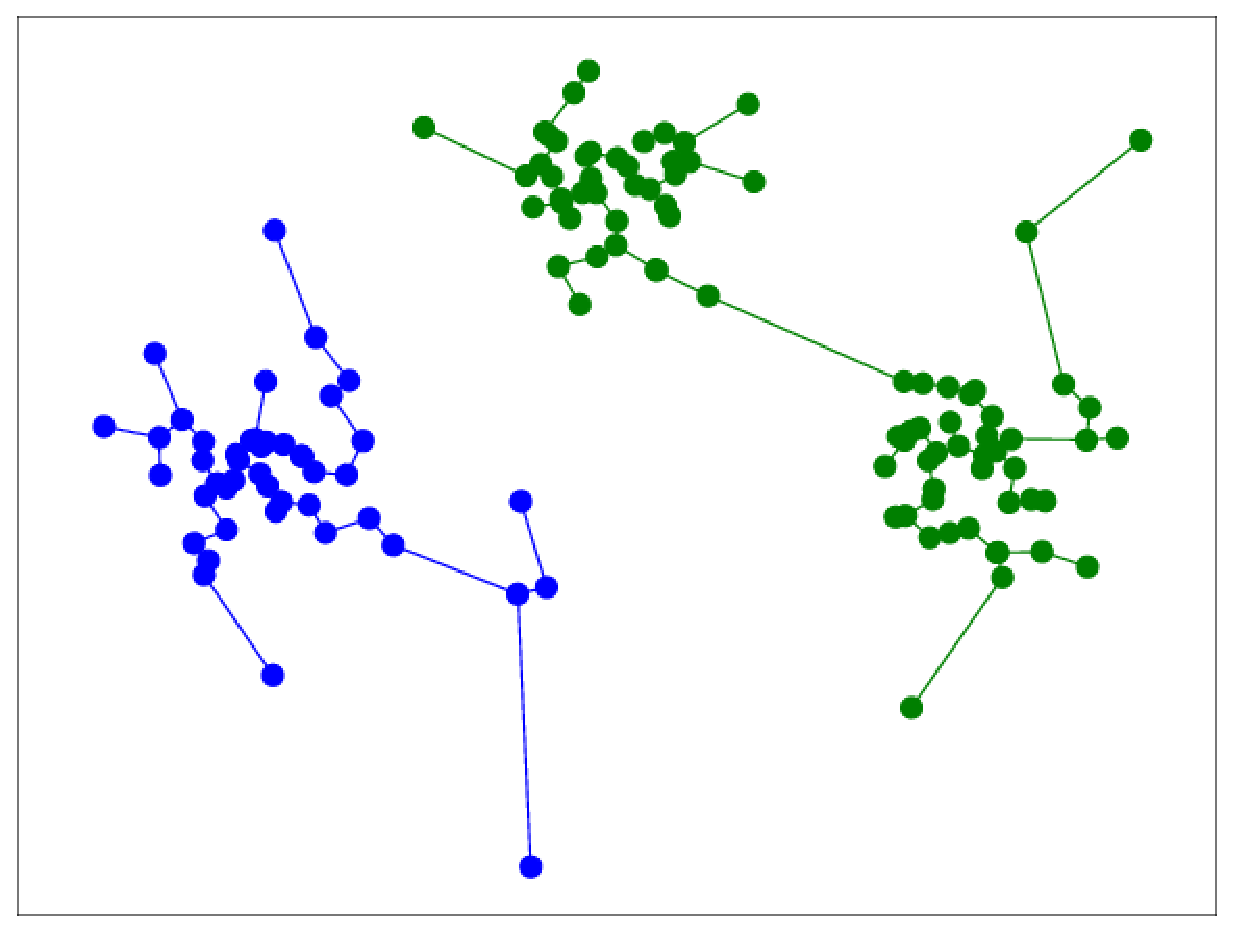
\includegraphics[width=.32\textwidth]{illustration_center}
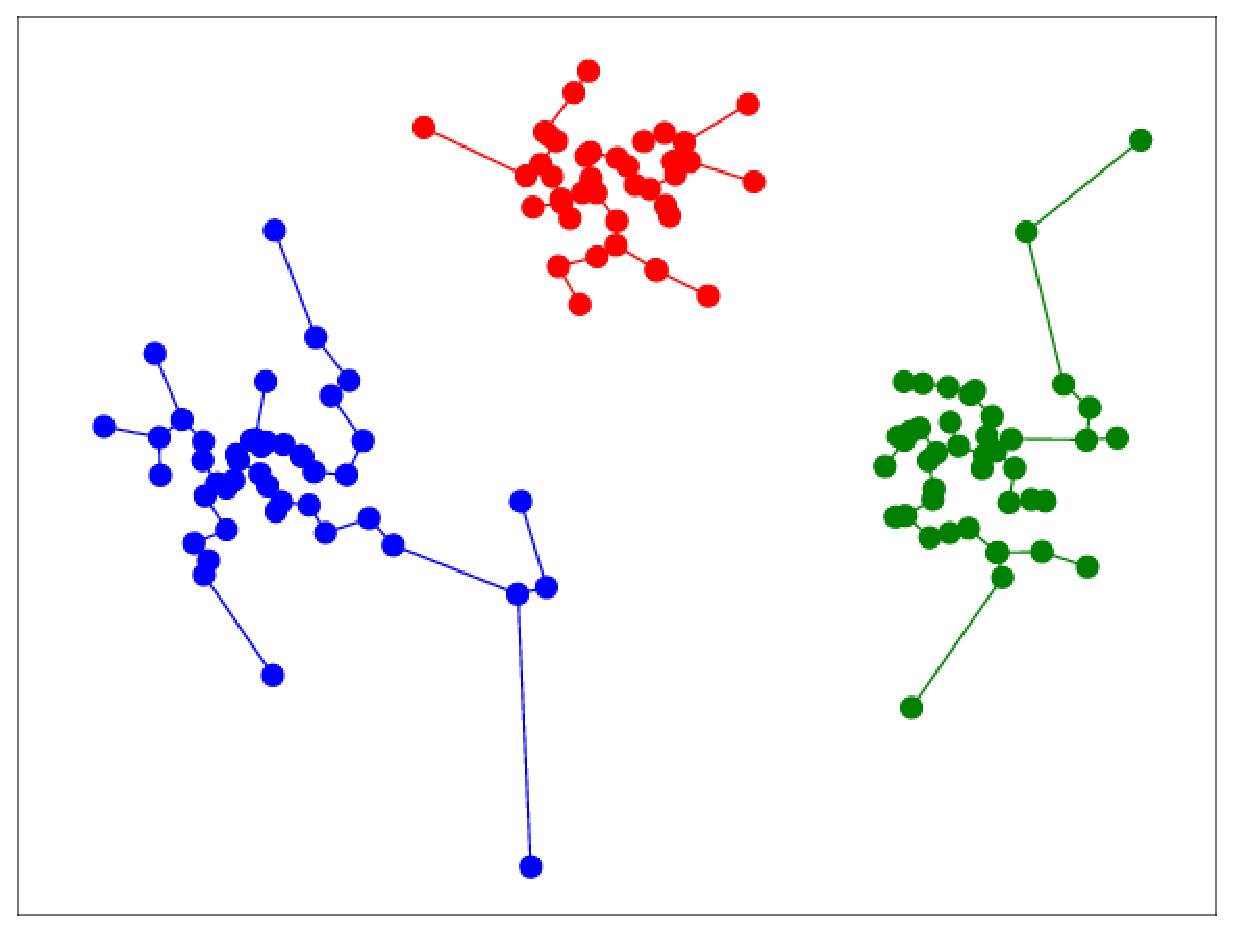
\includegraphics[width=.32\textwidth]{illustration_right}
\caption{Illustration of the optimization algorithm for $k=3$ on synthetic
dataset. \emph{Left}: Euclidean minimum spanning tree of the data.
\emph{Center}: The edge that yields the best two-cluster partition in terms of
\Eqref{objective} was removed, yielding two connected components. \emph{Right}:
Another edge from the forest was removed, resulting in the desired number of
three components. Note that the edges that are removed are not the longest edges
but form a trade-off between edge length and cluster size.}
\label{fig:illustration}
\end{figure}

\begin{algorithm}[t]
\begin{algorithmic}
    \Require Points $\mathbf{x}$, desired number of clusters $k$.
    \Ensure Clustering $\mathbf{y}$ of $\mathbf{x}$
    \State $G \leftarrow T(\mathbf{x})$
    \For{$i=0,\dotsc,k-1$}
        \For{$G_j, j=0,\dotsc, i$ connected components of $G$}
            \State $e_j \leftarrow \text{SplitCluster}(G_j)$
        \EndFor
        \State $l \leftarrow \displaystyle \argmax_j\  \hat{I}(G_j \setminus e_j)$
        \State $G \leftarrow G \setminus e_l$
    \EndFor
    \Statex
    \Function{SplitCluster}{$G$}
        %\Require Euclidean minimum spanning tree $T$, dimension $d$
        %\Ensure $e^* = \displaystyle \argmax_{e\in E(T)} \ \hat{I}(G \setminus e )$
        \State Pick arbitrary root $x_0$ of $G$.
        \For{node $x$ starting from leaves}
            \State $w_x \leftarrow \displaystyle \sum_{c \in \text{children}(x)} w_c + d(x, c)$
            \State $n_x \leftarrow \displaystyle 1 + \sum_{c \in \text{children}(x)} n_c$
        \EndFor
        \For{node $x$}
        \State $w'_x \leftarrow w_{x_0} - w_x$
        \EndFor
        \For{$e \in E(G), e=(c, p)$, $p$ parent of $c$}
            \State $v_c \leftarrow w'_p + w_p - w_c - d(p,c)$
            \State $m_c \leftarrow n - n_c$
            \State objective$(e) \leftarrow d m_c \ln(m_c) - (d-1) m_c \ln(v_c) + d n_c \ln(n_c) - (d-1) n_c \ln (w_c)$
        \EndFor
        \State $e^* \leftarrow \displaystyle \argmax_{e \in E(G)} \ \text{objective}(e)$
        
    \EndFunction
\end{algorithmic}
\caption{Information Theoretic MST-based Clustering\label{overall}}

\end{algorithm}

For the above reasons, we propose a simple procedure to approximately solve
\Eqref{objective}.
%filler removed Let us first fix some notation.
Consider a graph $G$ with nodes $\mathbf{x}$, an arbitray set of edges, and edge weights given by the
Euclidean distances between points.  The connected components of $G$ induce a
clustering $\mathbf{y}(G)$ of $\mathbf{x}$, by assigning $x_i$ and $x_j$ the
same cluster if and only if they are in the same connected component of $G$.
Define
\begin{align}\label{eq:graphobjective}
\hat{I}(G) := - \sum_{y=0}^k p(y) \Bigl[ d \log(L_{G,y}) - (d-1) \log{n_y} \Bigr],
\end{align}
where $y$ enumerates the connected components $G_0, \dotsc, G_k$ of $G$, $n_y =
|V(G_y)|$ is the number of nodes in $G_y$ and $L_{G,y} = \sum_{e \in E(G_y)}
w(e)$ is the sum of the weights of all edges in the connected component $G_y$.
%
Then $\hat{I}(G) \geq \hat{I}\bigl(\mathbf{y}(G)\bigr)$, by the definition of
the minimum spanning tree, and equality holds if and only if $G_y$ is the
minimum spanning tree of its nodes for all $y$.
%
We try to find a graph $G$ with $k$ components, such that $\hat{I}(G)$ is maximal. We can restrict
ourself to optimizing over the set $\mathcal{F}$ of forests over $\mathbf{x}$ with $k$ components,
as adding edges inside connected components only decrease the objective.
Thus we can formulate the clustering problem equivalently as
\begin{equation}
    \max_{G \in \mathcal{F}} \hat{I}(G).
\end{equation}
Optimization over forests remains hard, and we further restrict ourself to
solutions of the form $\mathcal{G} := \{ F \in \mathcal{F} \mid F \text{\ subgraph of\
} T(\mathbf{x}) \}$ for a given minimum spanning tree $T(\mathbf{x})$, leading to
the problem $\displaystyle \max_{G \in \mathcal{G}} \hat{I}(G)$.  This restriction allows for
a very fast, combinatorial optimization procedure.


For the two class case, optimization of the above objective can be solved
exactly and efficiently by searching over all of $\mathcal{G}$.
This amounts to searching for the edge $e$ that maximizes $\hat{I}\bigl(T(\mathbf{x})
\setminus e\bigr)$. The naive algorithm that computes the objective for each edge
separately has run time that is quadratic in the number of data points.  To
improve upon this, we use a dynamic programming approach as described in
function \textsc{SplitCluster} of Algorithm~\ref{overall} , which has only linear
complexity. Using this algorithm, run time in the two cluster case is dominated
by computing $T(\mathbf{x})$.
%
We extend this algorithm to the case of more than two clusters in a greedy way:
Starting with the full spanning tree of $\mathbf{x}$, we remove the edge
yielding the lowest value of \Eqref{graphobjective} until the number of
components equals the number of desired clusters. The overall procedure is
summarized in Algorithm~\ref{overall}, which we call \emph{Information
Theoretic MST-based (ITM) clustering}.  An illustration can be found in
\Figref{illustration}

We use Prim's algorithm combined with a ball tree data structure for distance
queries to compute the minimum spanning tree of the data.
While this procedure has no strong runtime guarantees, we found this faster
in practice than specialized algorithms for euclidean minimum spanning trees, 
which achieve a better theoretical runtime of $O\bigl(n \log(n) \alpha(n)\bigr)$ \citep{dtb2010}. Here
$\alpha$ is the inverse of the Ackerman function. The dynamic programming solution of
Algorithm~\ref{overall} has a run time of $O(n)$ per removed edge, leading to an overall
run time of $O\bigl(n \log(n) \alpha(n)+ nk\bigr)$. The $O(nk)$ comes from a worst case
scenario, in which each step in the hierarchical clustering procedure only
splits off a constant number of points. In a more realistic setting, we expect
that the individual clusters are much smaller than the original dataset. In
this case, the $O(nk)$ factor would improve to $O\bigl(n\log(k)\bigr)$.

\subsection{Estimating Intrinsic Dimensionality}
While assuming totally continuous densities is very natural from a theoretical
point of view, it can be a hindrance in practical applications.  Often, the
data is assumed to lie on a submanifold, embedded in a
higher-dimensional space. In this case, the density is not totally continuous,
and the dimensionality of the data can not be taken as the dimensionality of
the embedding space.

A particularly drastic example is the case of the dataset having less samples
than features. In this case, the data clearly lies even on a linear subspace
of the input space, and the dimensionality of the input space does not
accurately reflect the intrinsic dimensionality of the data.
We use the estimate analyzed in \citet{massoud2007manifold}.
In their method, for each data point $x$, a local estimate $\hat{d}(x)$ of the
dimensionality at $x$ is computed as
\begin{equation}
    \hat{d}(x) = \frac{\ln 2}{\ln\left(r_k(x) / r_{\lfloor k /2 \rfloor}(x)\right)}.
\end{equation}
Here $k$ is a fixed integer and $r_k(x)$ is the distance of $x$ from its $k$th neighbor.
We follow \citet{massoud2007manifold} and set $k =\lceil 2 \ln n\rceil$.
The final estimate $\hat{d}$ is then computed by averaging the estimates over all $x$
\begin{equation}
    \hat{d} = \frac{1}{n}\sum_{x \in X} \min\left(\hat{d}(x),\ d\right).
\end{equation}
We compute the density estimate once, prior to clustering, and then plug the
estimate $\hat{d}$ into \eqref{graphobjective} in place of $d$.
We found this estimate to work robustly and give sensible results for all
datasets we investigated. As we already used a ball tree data structure to
build the minimum spanning trees, we can reuse this structure to compute $r_k$.
Consequently, estimating the dimensionality resulted only in little
computational overhead.

\begin{figure}[t]
\centering
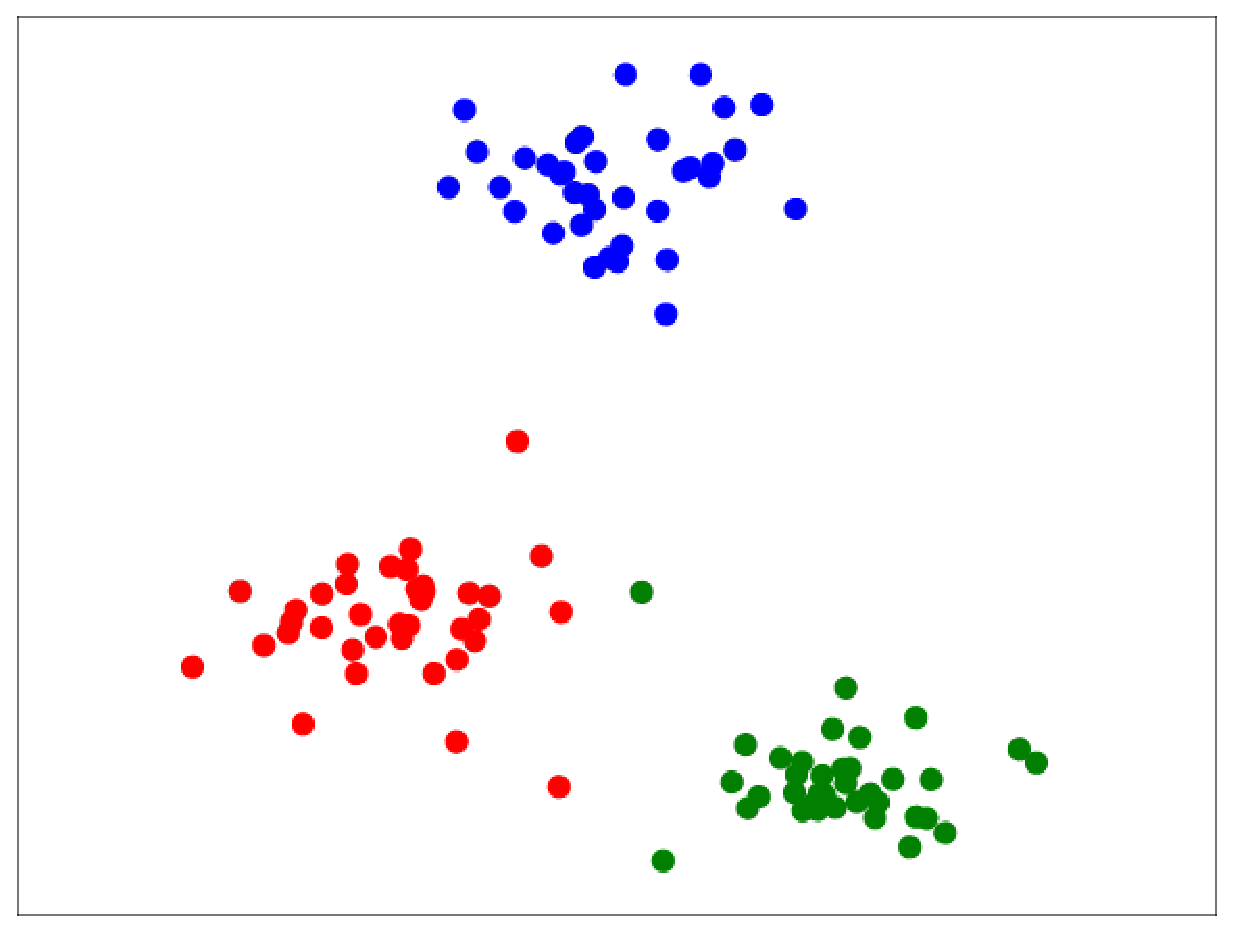
\includegraphics[width=.24\textwidth]{qualitative_blobs_km}
\includegraphics[width=.24\textwidth]{qualitative_blobs_mean_nn}
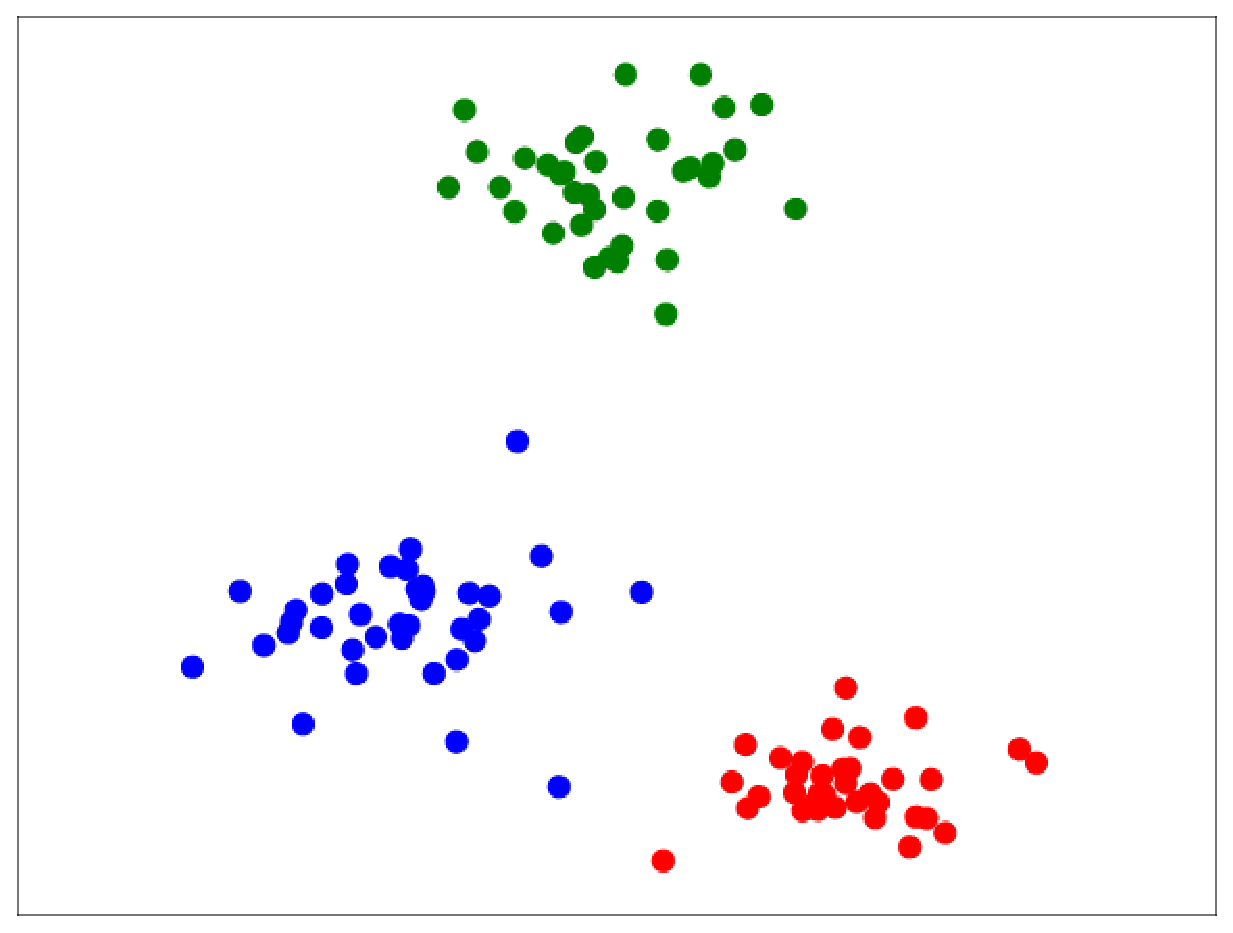
\includegraphics[width=.24\textwidth]{qualitative_blobs_aggl}
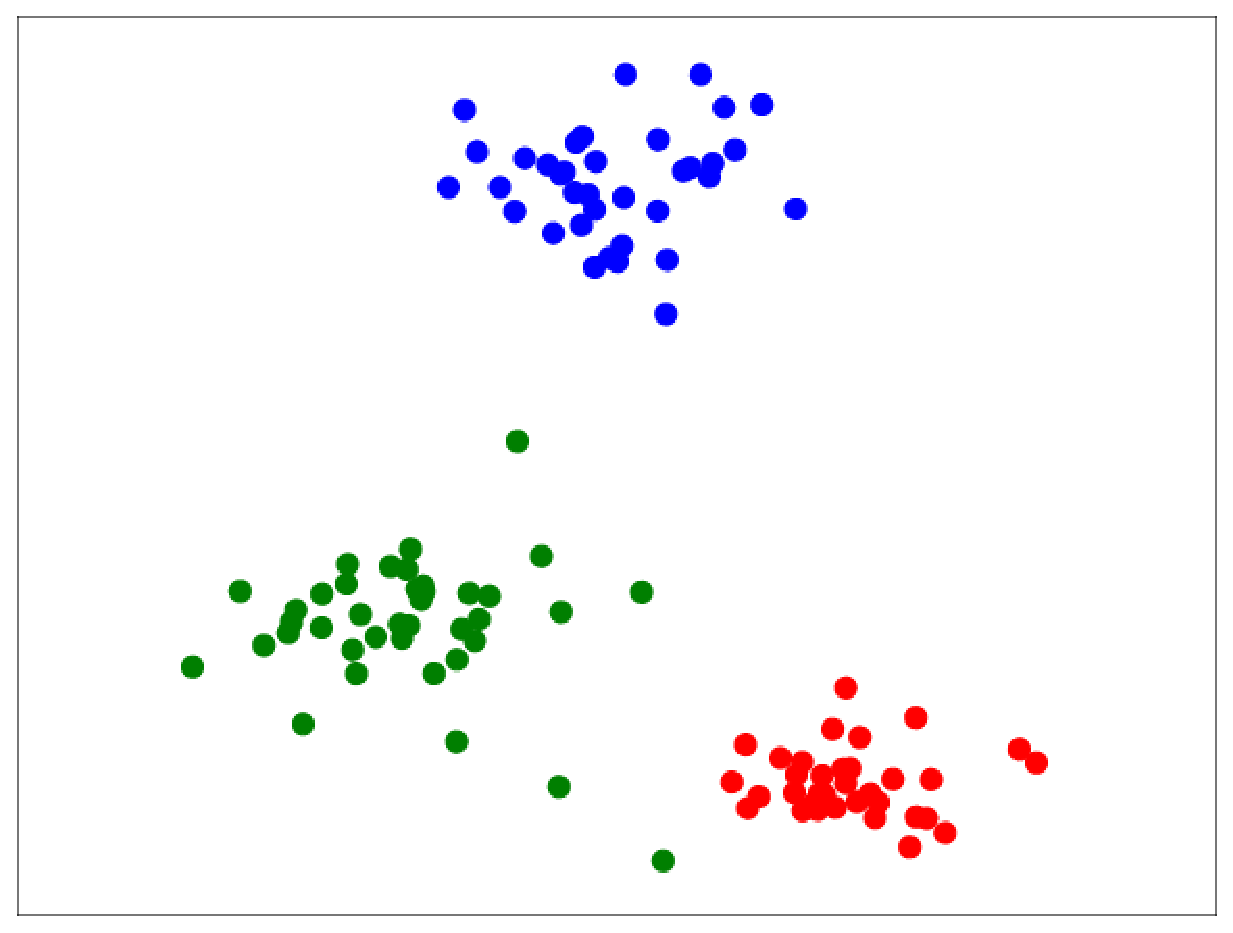
\includegraphics[width=.24\textwidth]{qualitative_blobs_mst} \\ 

\includegraphics[width=.24\textwidth]{qualitative_circles_km}
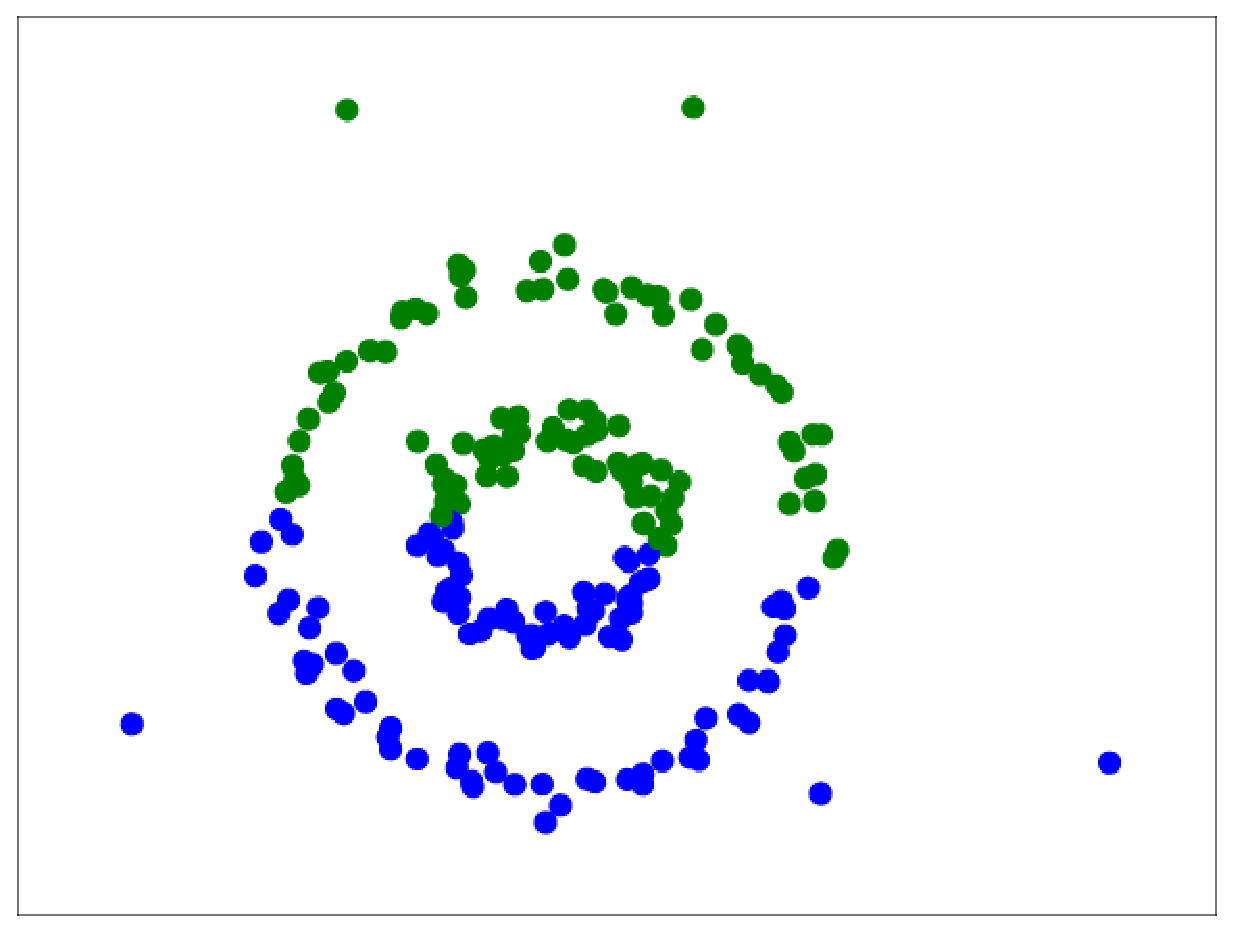
\includegraphics[width=.24\textwidth]{qualitative_circles_mean_nn}
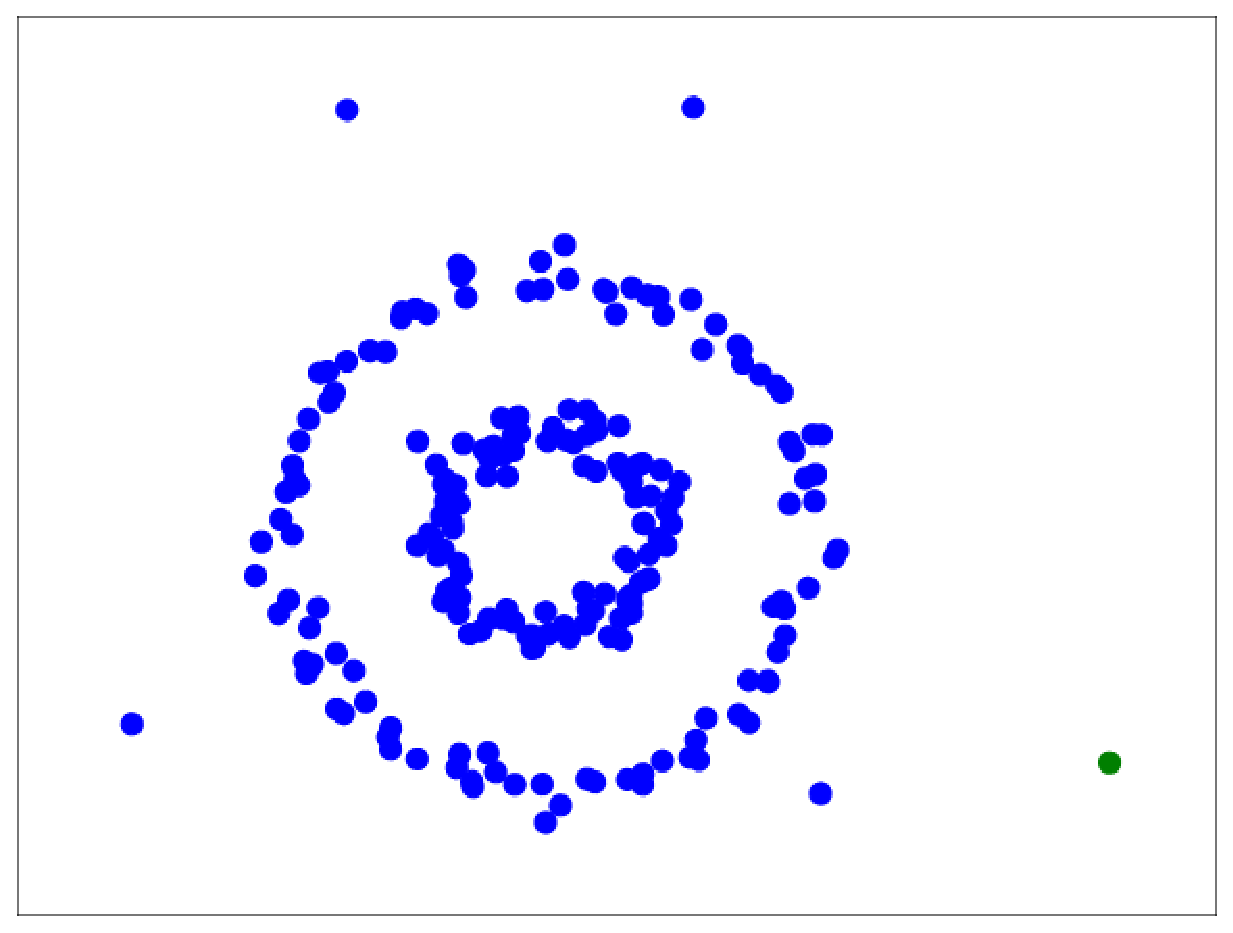
\includegraphics[width=.24\textwidth]{qualitative_circles_aggl}
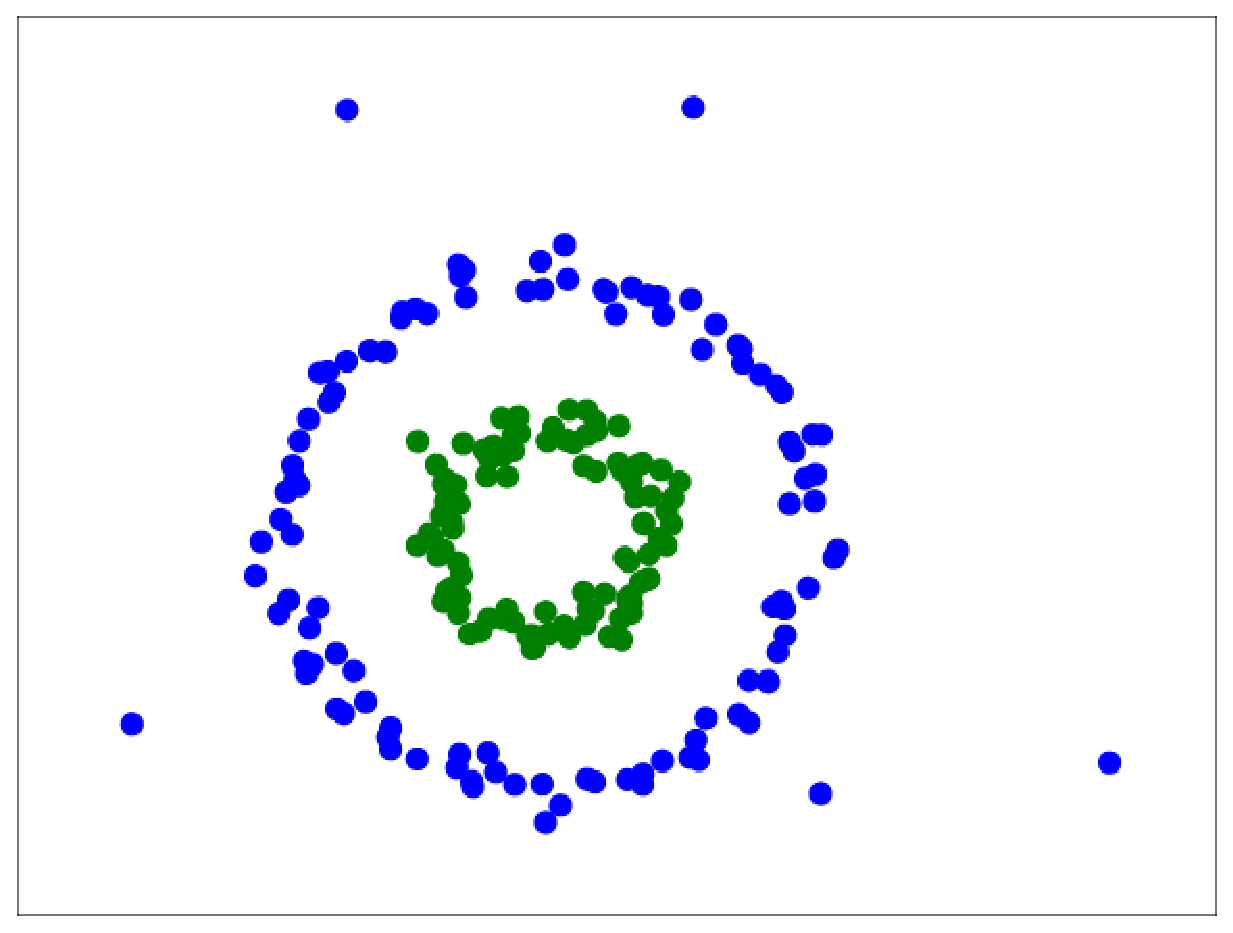
\includegraphics[width=.24\textwidth]{qualitative_circles_mst} \\ 

\includegraphics[width=.24\textwidth]{qualitative_circles2_km}
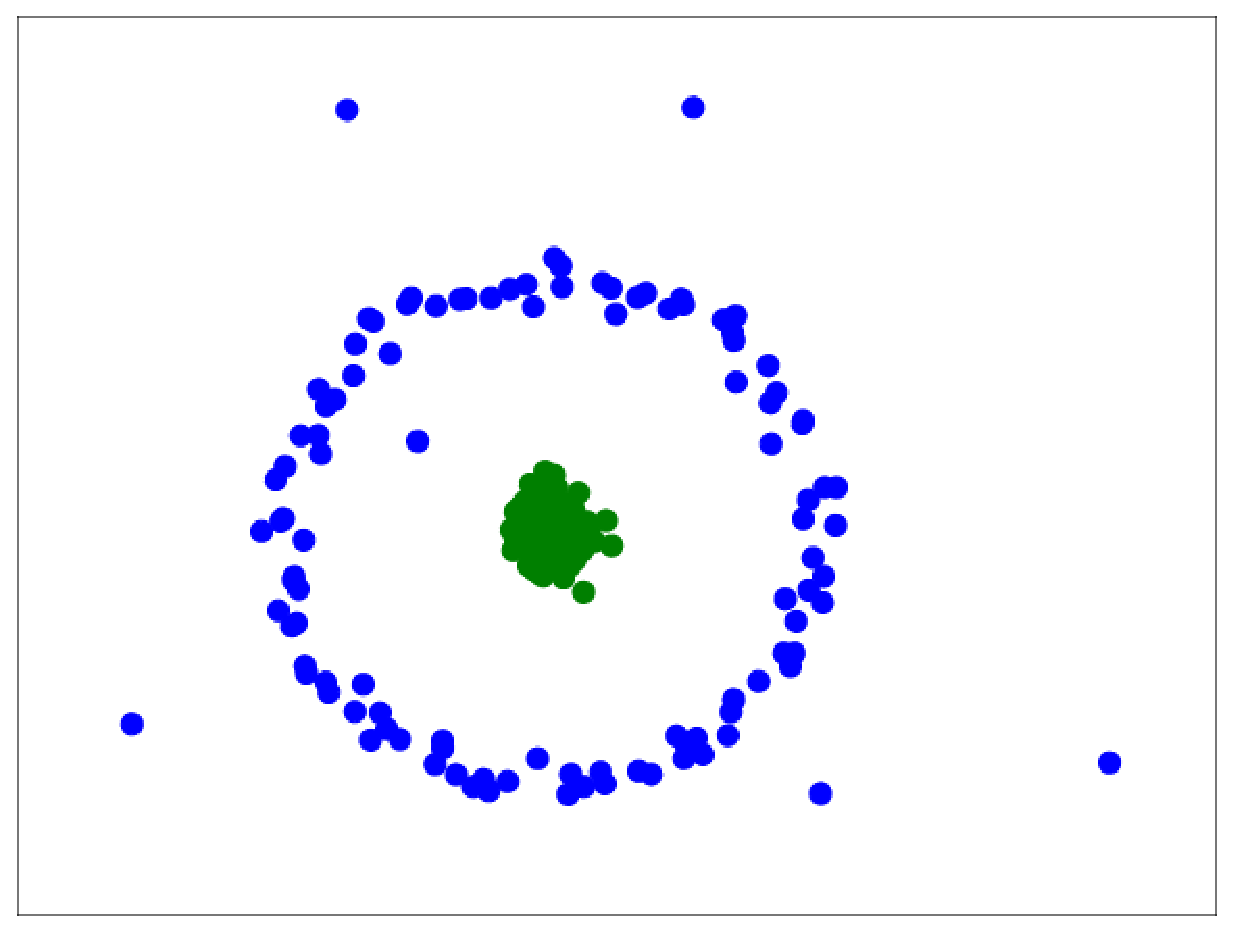
\includegraphics[width=.24\textwidth]{qualitative_circles2_mean_nn}
\includegraphics[width=.24\textwidth]{qualitative_circles2_aggl}
\includegraphics[width=.24\textwidth]{qualitative_circles2_mst} \\ 

\includegraphics[width=.24\textwidth]{qualitative_twomoons_km}
\includegraphics[width=.24\textwidth]{qualitative_twomoons_mean_nn}
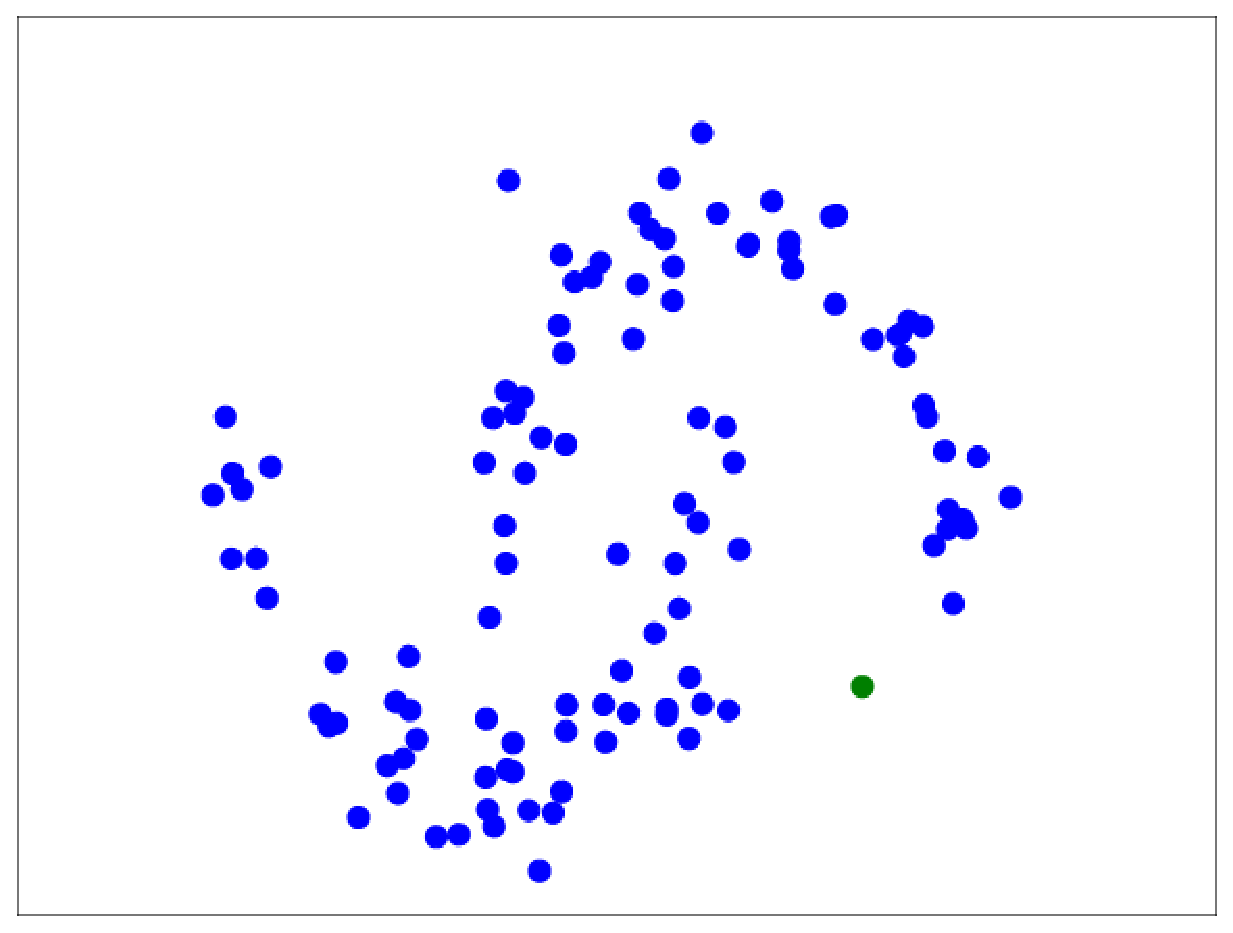
\includegraphics[width=.24\textwidth]{qualitative_twomoons_aggl}
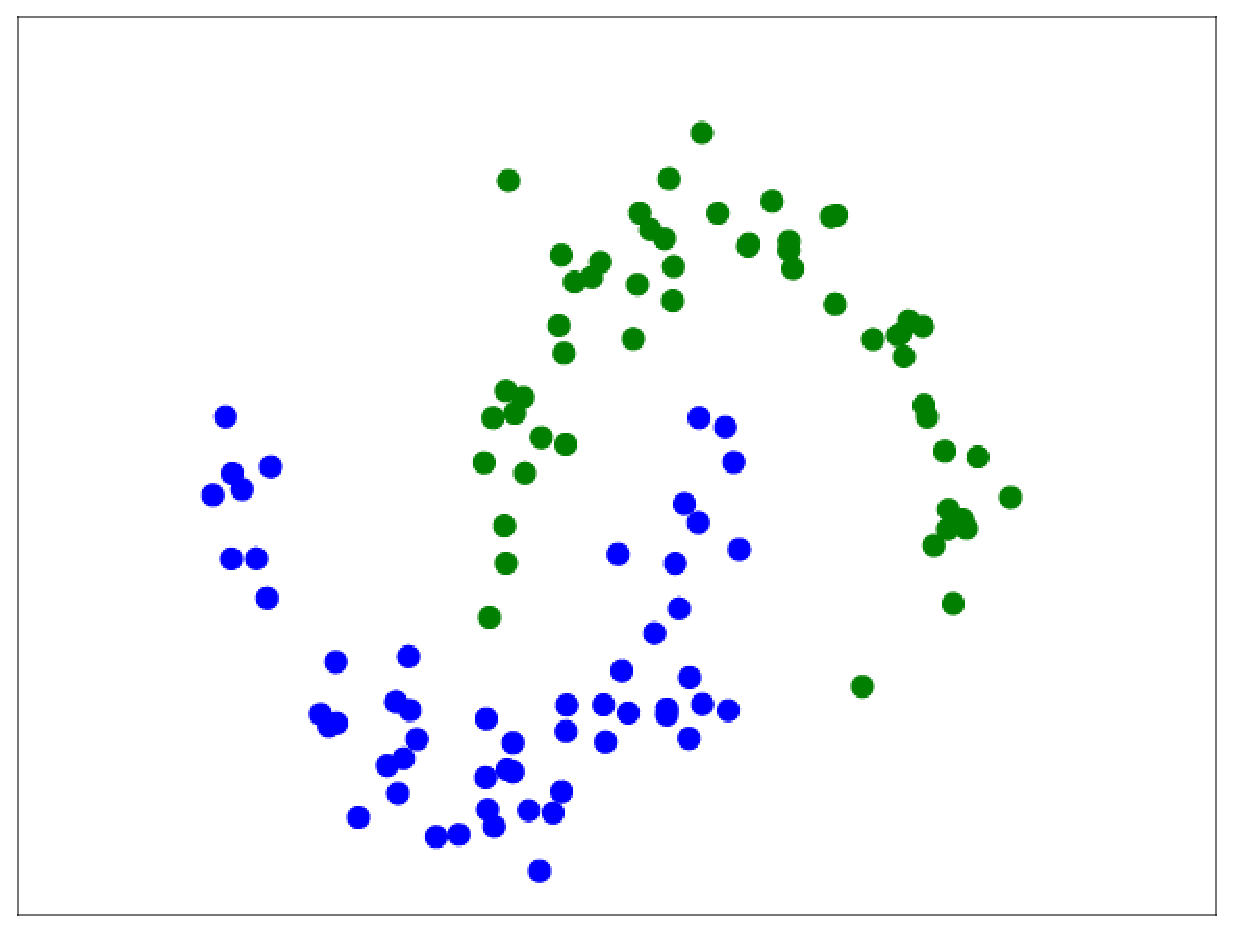
\includegraphics[width=.24\textwidth]{qualitative_twomoons_mst} \\ 
\caption{Comparison of $k$-Means (left), MeanNN (center left), single link
(center right) and ITM (right) on four synthetic datasets.  Without the need to
tune parameters, ITM can adjust to different cluster shapes.  MeanNN is able to
recover non-convex clusters (third row) but often produces similar results to
$k$-Means (second and last row). Single link clustering is very sensitive
to noise, as it does not take cluster size into account.}
\label{fig:qualitative}
\end{figure}

\section{Experiments}
We compared ITM to the popular $k$-Means algorithm 
\citep{macqueen1967some,lloyd1982least}, to the MeanNN algorithm of
\citet{faivishevsky2010nonparametric} and to single-link agglomerative
clustering~\citep{gower1969minimum}. The similarities between single-link
agglomerative clustering and the proposed MST-based optimization make it a 
good baseline for tree-based clustering approaches.

\enlargethispage{5mm}
A comparison of ITM, MeanNN and the baseline methods, $k$-Means and 
single link agglomerative clustering, in terms of their objective, 
optimization and complexity can be found in Table~\ref{nowotab}. 
We implemented the ITM clustering procedure as well as MeanNN in Python.  We
used the $k$-Means implementation available in the \textsc{scikit-learn}
library~\citep{pedregosa2011scikit}. The source
code is available online\footnote{\url{https://github.com/amueller/information-theoretic-mst}}.

\subsection{Experimental Setup}
For both $k$-Means and MeanNN, we restart the algorithm ten times using
different random initializations, keeping the result with the best objective
value. As ITM is deterministic there is no need for random restarts.  All of
the algorithms we compare work with a fixed number of clusters, which we set to
the number of classes in the dataset for all experiments.

As single link agglomerative clustering is sensitive to outliers, we set
a hard limit of five on the minimum number of samples per cluster for
the quantitative analysis.

\begin{table}[t]
\centering
\begin{tabularx}{\linewidth}{@{\extracolsep{\fill}}lccc}
\toprule
Algorithm &     Objective &     Det.&      Complexity \\
\cmidrule{1-4}
$k$-Means &     $\displaystyle \sum_y \sum_{i, y_i = y} \| x_i - \mu_y \|^2$ & No  & $O(nk)$ per iteration%
%\footnote{The worst-time complexity of the Lloyd-Algorithm is exponential~\cite{arthur2006slow}, though online algorithm are observed to converge in linear time~\cite{bottou1995convergence}.}
\\
MeanNN &    $\displaystyle \sum_y \log\left(\frac{1}{|\mathbf{x}_y|}\sum_{i,j, y_i=y_j=y} \| x_i - x_j \|^2 \right)$ & No & $O(n^2)$ per iteration\\
Single Link &   -- &    Yes    &    $O(n\log n)$\\
ITM & $\displaystyle \sum_{y=0}^k d p(y) \log(\bar{L}_y  ) + p(y) \log{p(y)}$ & Yes & $O\bigl(\alpha(n) n \log n + nk\bigr)$\\
\bottomrule
\end{tabularx}
\caption{Comparing properties of related algorithms. Det.\ stands for Deterministic}\label{nowotab}
\end{table}

%As our objective is motivated by limit properties of the entropy estimate of \Eqref{hmst},
%we expect the objective to work best in a setting with many samples. To avoid tautological
%solutions, we set a hard lower limit to the number of points in each cluster.
%This limit was set to $10$ for all experiments, independent of the number of samples and clusters.

\subsection{Qualitative Results}
\Figref{qualitative} shows qualitative results on three synthetic datasets.
For well separated, convex clusters, the four algorithms produce very similar
clusters (see top row).  If the structure of the data is more complex, the
advantage of the proposed method is apparent.  Note that there was no need to
specify any other parameters than the number of clusters to produce these
results.  It is also noteworthy that the results of MeanNN are very close to
those produces by $k$-Means in most cases. This similarity can be explained
by the close relation of the objective functions, listed in Table~\ref{nowotab}.

\subsection{Quantitative Results}
We present results on several standard datasets from the UCI repository, 
selecting datasets that span a wide range of combinations of number
of samples, features and clusters.
To satisfy the assumption of absolute continuity of the data distribution, 
we restrict ourself to data with continuous features.

We evaluated the experiments using the \emph{adjusted Rand index 
(ARI}~\citep{hubert1985comparing} a popular measure
of cluster quality~\citep{gomes2010discriminative,kamvar2003spectral}.
The Rand index~\citep{rand1971objective} between two clusterings counts on how
many pairs of points two clusterings agree. The adjusted Rand index contains a
calibration against chance performance.
We also measured \emph{normalized mutual information
(NMI)}~\citep{strehl2003cluster}, but do not report it here, as it resulted in
an identical ranking of the clustering algorithms.

Table~\ref{results} summarizes the results. The two entropy-based methods 
(MeanNN, ITM) have a clear advantage of the other methods, with ITM finding 
better clusterings than MeanNN in the majority of cases.
We see that ITM does well when the intrinsic dimensionality of the data matches
the feature dimension, but degraded otherwise (see ``faces'' and ``usps'').
Estimating the intrinsic dimensionality of the data overcomes this weakness,
and improves results in most cases. For all but one dataset, either ITM or ITM with
estimated intrinsic dimensionality gives the best results of all considered
algorithms.
%
The single link agglomerative clustering procedure produces reasonable 
results on datasets with little noise and well-separated clusters, but 
fails otherwise.
%
The run time of computing the ITM clustering was dominated by the computation
of the MST of the data.
%
% TODO runtime statements!
% One table datasets, one table methods + runtime?

\begin{table}[t]
\centering
\begin{tabularx}{\linewidth}{@{\extracolsep{\fill}}lrrrccccc}
\toprule
\multicolumn{4}{c}{Dataset} &\multicolumn{4}{c}{Results}\\
\cmidrule{1-4}
\cmidrule{5-9}
Description &     n &    d &   k &  $k$-Means      & MeanNN        & SL            &   ITM        & ITM ID \\
\cmidrule{1-4}                   \cmidrule{5-5}    \cmidrule{6-6}  \cmidrule{7-7} \cmidrule{8-8} \cmidrule{9-9}
digits      &$ 1797$&$  64$&$ 10$& $    0.62 $&     $0.67$           &$0.10$         &$\mathbf{0.85}$       &$0.73$\\ 
faces       &$  400$&$4096$&$ 40$& $    0.41 $&     $0.49$           &$0.08$         &$0.02$           &$\B{0.54}$\\ 
iris        &$  150$&$   4$&$  3$& $    0.72 $&     $0.75$           &$0.55$         &$\B{0.88}$       &$0.88$\\
usps        &$ 9298$&$ 256$&$ 10$& $    0.52 $&     $0.54$           &$0.00$         &$   0.44$        &$\B{0.64}$\\ 
vehicle     &$  846$&$  18$&$  4$& $    0.10 $&     $0.09$           &$0.00$         &$\B{0.10}$       &$0.10$\\
vowel       &$  990$&$  10$&$ 11$& $    0.17 $&     $0.19$           &$0.00$         &$\B{0.20}$       &$0.19$\\
waveform    &$ 5000$&$  21$&$  2$& $\B{0.37} $&     $0.30$           &$0.00$         &$   0.23 $       &$0.23$\\
mnist       &$70000$&$ 784$&$ 10$& $    0.37 $&     N/A$^\dagger$    &$0.00$         &$   0.50$        &$\B{0.77}$\\
\bottomrule
\end{tabularx}
\caption{Adjusted Rand Index of $k$-Means, MeanNN, single link agglomerative
    clustering and ITM on several datasets (higher is better). ITM ID refers to
    ITM using the estimated intrinsic dimensionality. The best score for each
    dataset is printed in bold.\\$^\dagger$\footnotesize We were unable to make
    MeanNN scale to 70000 data points, as storing the whole pairwise distance
    matrix seems necessary.\label{results}}
\end{table}

% TODO more experiments: mnist
% todo segmentation unsupervised
% TODO bag of word experiment?
% report times on experiments?

\section{Summary}
In this chapter we proposed the use of a minimum spanning tree based,
non-parametric entropy estimator in information theoretic clustering, ITM\@.
Thereby we extended the work of \citet{faivishevsky2010nonparametric} to a more
flexible and efficient entropy estimate.  We proposed an approximate optimization
method by formulating the clustering problem as a search over graphs.
The resulting algorithm is deterministic and has sub-quadratic run time.
%
Empirical comparisons showed that the proposed method outperforms standard
algorithms and the non-parametric entropy based clustering of
\citep{faivishevsky2010nonparametric} on multiple benchmark datasets. We
demonstrated that ITM is able to detect non-convex clusters,
even in the presence of noise.
%
In contrast to other algorithms that can handle non-convex clusters, ITM has no
tuning parameters, as the objective presents a natural trade-off between
balancing cluster sizes and enforcing intra-cluster similarity.
%
A limitation of the proposed algorithm is that it is based on the assumption 
of an absolute continuous data distribution. We show that this limitation can
be overcome in practice by estimating the intrinsic dimensionality of the data. 
%
%In future work we plan to investigate a way to overcome this limitation, 
%for example by estimating the intrinsic dimensionality of the 
%data~\citep{pettis1979intrinsic}.
%
%We also investigate optimizations of the objective 
%\Eqref{graphobjective} that go beyond the proposed method. 
%Move-making algorithms seem a promising way to refine solutions 
%found by Algorithm~1. Branch and bound techniques could provide 
%an alternative approach. 


\chapter{Weakly Supervised Object segmentation via Multiple Instance Learning}
In this work, we explore the 
application of multi-instance learning algorithms to the task of partially supervised image segmentation.
Multi-Instance learning is a natural formulation for image classification and has been
successfully applied in this task~\cite{zhou2007multi}. We propose to go a step further and apply
multi-instance learning to the task of object class segmentation in natural
images.  In object class segmentation, the goal is to create a pixel-wise
labeling of an input image into one of several semantic
classes.  Multi-class image segmentation receives much attention in the
computer vision community at the moment. To our knowledge, all previous
methods in the field use strong supervision, meaning manual pixel-wise annotation of
training images. This approach does not
scale to larger datasets, especially if one expects consistency and quality
in the segmentations.

In this work, we investigate the use of multi-instance
learning to obtain multi-class image segmentations using ground truth labeling
only on the image level.
We focus on the multi-class, single label setup, where each image is assigned
one of multiple classes. We formulate multi-class image segmentation as
a multi-instance learning problem by considering each image as a bag of
overlapping candidate segments. 

The standard multi-instance setup is as follows. Let $\mathcal{X}$ be a set of
instances. Then a bag is an element of the power set $2^\mathcal{X}$ and the
task is to learn a function
%\begin{equation}
$f_{MI} \colon 2^\mathcal{X} \rightarrow \{-1,+1\}$
%\end{equation}
from a set of training examples of the form $(X_i,y_i)$ with
bags $X_i \subset \mathcal{X}$ and labels $y_i \in \{-1,+1\}$.  This function
stems from the so-called underlying concept, given by an (unknown) function
$f_{I} \colon \mathcal{X} \rightarrow \{-1,+1\}$, with 
\vspace{-3mm}
\begin{equation}\eqlabel{multi_instance}
f_{MI}(X)= \max_{x \in X} f_{I}(x).
\vspace{-3mm}
\end{equation} 
%In our case, instances are overlapping segments, obtained using constraint
%parametric min-cuts~\cite{carreira2010constrained}.  Each image is a bag
%consisting of hundreds of these segments.
Sometimes, the goal of finding $f_{MI}$ is extended to finding labels not only
on bag-level but also for all the instances within a bag
\cite{liconvex2010,zha2008joint}, i.\ e.\ finding $f_{I}$.\\ 
Even though finding $f_{I}$ is sometimes included in the task statement, there
has been very little work that actually reported accuracy on instance-level. Part
of the reason for this might be that for many of the datasets used in
multi-instance learning no ground truth exists.

We look explicitly at accuracy on instance-level since we are interested in
actually segmenting images, not just classifying them. For multi-class image
segmentation, there are some hand-labeled datasets that provide ground truth
on pixel-level. We use this ground truth to evaluate the performance of our
method. This does not exactly correspond to instance-level ground truth --
since the instances are segments, not pixels -- but relates to it closely.

Since scalability is very important in real-world computer vision
applications, and natural images might need hundreds of segments to
account for all possible object boundaries, we use the efficient
multi-instance kernels~\cite{graetner2002multi}.
Multi-instance kernels are a form of set kernels that transform a kernel
on instance-level to a kernel on bag level.
With $k_I$ denoting a kernel on instances $x,x' \in \mathcal{X}$, we define the
corresponding multi-instance kernel $k_{MI}$ on bags $X,X' \in 2^\mathcal{X}$
as 
\vspace{-2mm}
\begin{equation}
    \eqlabel{mi_kernel}
    k_{MI}(X,X') := \sum_{x \in X, x' \in X'} k^p(x,x'),
\vspace{-2.5mm}
\end{equation}
where $p \in \mathbb{N}$ is a parameter.  As we use the RBF-kernel
$k_{rbf}$ as kernel on $\mathcal{X}$ and powers of RBF-kernels are again
RBF-kernels, we will not consider $p$ in the following.
We normalize the kernel $k_{MI}$ in feature space.

%\begin{equation}
    %k(X,X') := \frac{k_{MI}(X,X')}{\sqrt{k_{MI}(X,X)k_{MI}(X',X')}}.
%\end{equation}
Training an SVM with this kernel produces a bag-level classifier for each class, which we will refer to as MIK.
This procedure is very efficient since the resulting Gram matrix is of size
number of bags, which is much smaller than a Gram matrix of size number of
instances, as is commonly used in the
literature~\cite{andrews2003support,nguyen2010new,zhang2008m3miml}.  Another
advantage over other methods is, that it uses a single convex optimization,
whereas other approaches often use iterative algorithms~\cite{andrews2003support} or need to fit complex
probabilistic models~\cite{zha2008joint}.

While using MIK has many advantages, it produces only an instance-level
classifier. We propose to transform a bag lavel classifier $f_{MI}$ as given by
the SVM and \eqref{mi_kernel} into an instance-level classifier by setting
$f_{I}(x):=f_{MI}(\{x\})$, in other words, by considering each instance as its own
bag. 

To assess the validity of predictions made by $f_{I}$, we transform it
back to an instance-level classifier, using the multi-instance learning
assumption \eqref{multi_instance}. We refer to these instance-based MIK predictions
as MIK-instance. In all experiments, the parameters of the MI-Kernel
and SVM are adjusted using MIK and then used with both MIK and MIK-instance.
This facilitates very fast parameter scans since MIK is very efficient to
compute.

\begin{table}
    \centering
    \vspace{-4mm}
    \begin{tabularx}{0.9\linewidth}{@{\extracolsep{\fill}}lccccccc}
    \toprule
        & SVM-SVR & EMDD & mi-SVM & MI-SVM & MICA & MIK & MIK-instance \\
    \cmidrule(rl){2-8}
    Musk1 & 87.9 &84.9 &  87.4 &  77.9     & 84.3 & 88.0& 88.0 \\
    Musk2 & 85.4 &84.8 &  83.6 &  84.3     & 90.5 & 89.3& 85.2 \\
    \bottomrule
    \end{tabularx}
    \vspace{1mm}
    \caption{Bag level performance of various MIL algorithms on the standard Musk
    datasets. All but MIK provide instance-level labeling. }
    \vspace{-8mm}
    \tablabel{musk-acc}
\end{table}
We compared the performance of MIK, MIK-instance and state-of-the-art MI
methods on the Musk benchmark datasets~\cite{dietterich1997solving}, see
\tabref{musk-acc}. Results were obtained using 10-fold
cross-validation. While the computational complexity of MIK-instance is
very low compared to the other methods, it achieves competitive results.
Using instance-level labels results in a slight loss of accuracy of
MIK-instances, compared to MIK\@. This small degradation of performance is quite surprising, since the model was
not trained to provide any instance-level labels.

For multi-class image segmentation, it is beneficial to have a low witness
rate, i.\ e.\ only a few instances are assumed to be positive in a positive
bag. Since an object might not be very prominent in an image, only a fraction
of segments might correspond to the object.
\tabref{musk-witness} compares the witness rates of MIK-instance,
miSVM~\cite{andrews2003support} and SVR-SVM~\cite{liconvex2010} on the Musk
datasets. MIK-instance is able to achieve similar accuracy
with much less witnesses than the other methods.  Note that Musk1 consists of
very small bags while Musk2 contains significantly larger bags, more similar to the
image/segment setup.
\begin{table}
    \centering
    \vspace{-6mm}
    \begin{tabularx}{.8\linewidth}{@{\extracolsep{\fill}}lcccc}
    \toprule
    & \multicolumn2c{Musk1}  & \multicolumn2c{Musk2}  \\
                &accuracy & witness-rate & accuracy & witness-rate  \\
    \cmidrule(rl){2-3}
    \cmidrule(rl){4-5}
    mi-SVM      & 87.4          & 100\%               &  83.6          & 83.9\%\\
    SVM-SVR     & 87.9          & 100\%               &  85.4          & 89.5\%\\
    MIK-instance& 88.0          & 99\%                &  85.2          & 62.3\%\\
    \bottomrule
    \end{tabularx}
    \vspace{1mm}
    \caption{MIL algorithms and the empirical witness rates of the
    classifiers.}
    \vspace{-10mm}
    \tablabel{musk-witness}
\end{table}
%The MIK-instance method can be extended to the multi-class setup using a
%straight-forward 1-vs-all strategy.
We evaluate the performance of the proposed algorithm for image class
segmentation on the challenging Graz-02 dataset.
This dataset contains 1096 images of three object classes, bike, car and person.
Each image may contain multiple instances of the same class.
From each image, we extract overlapping object-like segments using constraint
parametric min cuts (CPMC,\cite{carreira2010constrained}). We use the top 200 ranked segments and discard the
rest.
Each segment is described using SIFT~\cite{lowe2004distinctive} and
ColorSIFT~\cite{van2009evaluating} features, from which we compute bag of
visual word histograms as well as histograms of oriented
gradients~\cite{dalal2005histograms}. We construct one MI-Kernel per
feature which are combined using multiple kernel learning.
We adjusted parameters on a hold-out validation set and used the
training and test sets as given by the dataset.
It is straight-forward to extend the binary MIK method to the multi-class
setting using a one-vs-all strategy.
We train one MKL-SVM per class using MIK and predict class labels on segment level
using MIK-instance. If at least one SVM classifies a segment as positive,
it is associated with the most confident class. Otherwise it is assigned
``background'' or no class.
This yields a classification of each segment into one of car, bike, person
or background. We merge segments into pixel-level class labels by setting
the label $y_x$ of a pixel $x$ according to
\vspace{-3mm}
\begin{equation}
    y_x = \text{argmax}_{y \in Y} \frac{\#\{S_i | p \in S_i \land y_{S_i}=y \}}{
    \#\{S_i | p \in S_i \}},
\vspace{-3mm}
\end{equation}
where $Y= \{$car, bike, person$ \}$, $S_i$ enumerates all segments within an
image and $y_{S_i}$ is the label of segment $S_i$. In words: each pixel is
assigned the class with the highest ratio of class segments vs non-class
segments containing it.

\begin{table}
    \centering
    \vspace{-6mm}
    \begin{tabularx}{0.8\textwidth}{lRRR}
    \toprule
                & car & bike & person \\
    \cmidrule(l){2-2}
    \cmidrule(l){3-3}
    \cmidrule(l){4-4}
        Pixel-level accuracy&   19.1\%&  27.7\%&  24.6\% \\
    \bottomrule
    \end{tabularx}
    \vspace{1mm}
    \caption{Pixel-level accuracy on the Graz-02 dataset.}
    \vspace{-8mm}
    \tablabel{graz}
\end{table}
If the ratio $\frac{\#\{S_i | p \in S_i \land y(S_i)=y \}}{\#\{S_i | p \in S_i \}}$ 
is smaller than $0.5$ for all labels, i.\ e.\ for all labels there are more
non-class segments than class segments at a given pixel, the pixel
is assigned to the background.
Per-class pixel accuracies are reported in \tabref{graz}, some qualitiative results are shown in \figref{results}. The overall
accuracy on images labels, which is the task that was actually trained, is $87\%$.
While the performance of our multiple-instance based approach is far
from current methods that use pixel-level annotations, whose pixel-level accuracy is around $70\%$~\cite{fulkerson2009class} on pixel-level,
it can serve as a baseline for research on weakly supervised methods for image segmentation..
\begin{figure}[tbp]
	\begin{center}
        \includegraphics[width=28mm]{images/car1_img.png}\hspace*{0.7ex}
        \includegraphics[width=28mm]{images/car1_gt.png}\hspace*{0.7ex}
        \includegraphics[width=28mm]{images/car1_pos.png}\hspace*{0.7ex}
        \includegraphics[width=28mm]{images/car1_neg.png}\hspace*{0.7ex}\\
        \vspace{1mm}
        \includegraphics[width=28mm]{images/person1_img.png}\hspace*{0.7ex}
        \includegraphics[width=28mm]{images/person1_gt.png}\hspace*{0.7ex}
        \includegraphics[width=28mm]{images/person1_pos.png}\hspace*{0.7ex}
        \includegraphics[width=28mm]{images/person1_neg.png}\hspace*{0.7ex}
	\end{center}
        \vspace{-7mm}
        \caption{Qualitative resultson on the Graz-02 dataset. Top: Results on
        category ``car''. Bottom: Results on category ``person''. From left to
        right: original image, ground truth segmentation, segment votes for
        correct class, segment votes against correct class (red many, blue few votes).}
	\figlabel{results}
        \vspace{-7mm}
\end{figure}

\section{Introduction}\seclabel{intro}
Multiple instance learning is a supervised learning scenario first proposed by \citet{dietterich1997solving}.
In multiple instance learning, examples are multi sets of instances, called bags, and each bag is assigned a class label.
It is assumed that each instance has a true label, defined by an underlying concept. The label of a bag is positive, if and only if one of
the instances it contains is labeled positive. The true label of instances is assumed to be unobserved by the learner who only has access to bag labels.

In the original formulation of multiple instance learning, the goal of the learner
was to predict the label of bags. Some recent works also aim at predicting
the label of individual instances, a much harder problem.
This can be viewed as learning an instance-level classifier using a form of weak supervision.

Learning to predict instance labels has been attempted in some recent work~\citep{liconvex2010,zhang2002dd}
but there has been very little theoretical study when and to which extend this is possible.
In this work, we explore which assumptions about the distributions of instances and labels
are necessary to learn instance-level classifiers from bag labels only.
We provide bounds on the instance label prediction error based on the
bag label prediction error. The bounds can be used to judge a learner when no
instance labeling exists for training or testing.
%If one is interested in classifying instances, such a bound is very important.
There are two applications that we target:
\begin{description}
\item[Setting 1:] Bag labels for a validation set are known and instance predictions need to be judged.
\item[Setting 2:] Bag labels for a test set can be bound using standard learning theoretic bounds and instance
predictions need to be judged.
\end{description}
The first case is very common in practical settings, where
cross validation is often used to set parameters of a predictor. This is
particularly important in support vector machines (SVMs) which are a popular
learning method for multiple instance problems~\citep{andrews2003support}.
If no instance labels are present for training, it is only possible to
choose parameters to minimize bag prediction error, which might be suboptimal if one
wants to minimize instance label misclassification. 
The bounds can also be used to find the amount of positive instances in positive bags,
known as the witness rate, which is an integral part of established multiple
instance algorithms~\citep{zhang2002dd,liconvex2010}.
The second case can be used to convert established bounds on the bag prediction error
to instance prediction error.

We show that it is possible to bound instance prediction error without
ever observing any instance labels even in fairly unrestricted settings.
To the authors knowledge, this is the first result of this kind.

Detailed proofs of all propositions can be found in the appendix.

\section{Related Work}
The theoretical analysis of multiple instance learning started with \citet{auer1997approximating} and later \citet{blum1998note}.
These works assume that instances are drawn i.i.d.\ from a single distribution over instances. Blum and Kalai showed that in this
setting, if the underlying concept is PAC-learnable in polynomial time, then the multiple instance learning problem is PAC-learnable
in polynomial time. Auer et\,al.\ showed that if there is an algorithm to PAC-learn multiple instance learning with axis-parallel
rectangles that is polynomial in size of the bag and dimension of the instance features, then it is possible to polynomially
PAC-learn DNF-formulars, a problem that is solvable only if $\text{RP}=\text{NP}$.
Recently, \citet{sabato2009homogeneous,DBLP:journals/corr/abs-1107-2021} proved bounds on the VC dimension and
fat shattering dimension of multiple instance learners by the corresponding dimension for a base learner.

All of the results above only consider predicting bag labels. There has been very little theoretical work
on predicting instance labels. In spite of the large amount of research on multiple instance learning algorithms 
(for example \citet{andrews2003support,gaertner2002multi,zhou2009multi,li2009convex,zhang2002dd,mangasarian2008multiple,leistner2010miforests,chen2006miles})
to the authors knowledge, the only quantitative evaluations of predicting
instance labels are by \citet{gehler2007deterministic} and by \citet{liconvex2010}. While these works show promising results,
no analysis of instance label prediction is given.

Sabato et\,al.\ also studied multiple instance learning as a way
to reduce labeling complexity~\citep{sabato2010reducing}.
In the setting of reducing label complexity, the learner creates
the bags itself. The instances can therefore be assumed to be globally i.i.d.\ and
the distribution of labels inside the bags is known a priori.
Under these assumptions, the instance label prediction error is bound using the bag label error.
This result is used to evaluate the sample complexity of learning from bags using empirical risk minimization.
In this work, we generalize some results from \citet{sabato2010reducing} to the setting where the distribution
of instance labels is unknown and to cases where instances inside a bag may be dependent.

\section{Preliminaries}
Throughout this work, $\mathcal{X}$ denotes the space of all instances. Bags are multi sets of instance $X=\{x_1,\dotsc, x_r\}$.
As usual in supervised learning tasks, we assume our training examples ($X_i,Y_i)$ to be i.i.d.\ from an unknown distribution.
We denote the label of an instance $x_i$ by $y_i$ and the label of the bag $X_i$ as $Y_i = \max\{y_j | x_j \in  X_i\}$.
We assume the bag size $r\in \mathbb{N}$ to be constant over all bags in a given problem. This restriction simplifies the treatment
significantly while our results can in great parts be carried over to settings with varying bag sizes.
We consider arbitrary classifiers $h_I\colon \mathcal{X} \rightarrow \{0, 1\}$ with associated bag classifier
$h_B(X) = \max \{h(x_1),\dotsc,h(x_r)\}$.
The goal is to learn a classifier $h$ which minimizes expected instance misclassification, given training bags and bag labels
$X_i$ and $Y_i$.
We do not consider specific hypotheses classes but instead try to bound the expected error of $h$ using the expected error of $h_B$.
During all of this work, we assume that the true instance labels are never observed.
We use the following notation: $p(h_I(x)=0):= h_0$, the negative rate of the classifier,
$p(h_I(x) \neq y) := e_I$, the instance error, and $p(h_B(X) \neq Y) := e_B$, the bag error.

\section{Necessary Assumptions}\seclabel{assumptions}
If we allow instances inside bags and their labels to have arbitrary dependencies, we are trying to find
$y_1,\dotsc,y_r$ maximizing $p(y_1,\dotsc, y_r | x_1, \dotsc, x_r)$. This is a structured 
prediction problem for which there is no hope solving it, given only bag labels.
Therefore, as usual in multiple instance learning, we assume there is an underlying concept for instances,
i.\,e.\ the label of each instance depends only on this instance.
In other words, we assume $p(y_1,\dotsc, y_r | x_1, \dotsc, x_r)=p(y_1|x_1) \cdot p(y_r|x_r)$.

If we allow arbitrary dependencies between the instances $x_i$ in a given bag, there is a simple example 
\citep{sabato2009homogeneous} that shows that learning instance classification is not necessarily possible.
Let $\mathcal{X}$ consist of two
distinct points $x_1$ and $x_2$ with corresponding labels $y_1 = 1$ $y_2 = -1$. If the distribution
of instances inside bags is such that each bag either contains two copies of $x_1$ or both of $x_1$ and $x_2$, then
by predicting all bags as positive, one can obtain a perfect bag classifier, while it is impossible to say anything
about the label of $x_2$.
Therefore, we need to make additional assumptions about the distribution of instances inside bags to enable
predicting instance labels.

\section{Independent Case}\seclabel{iid}
The simplest case in which learning instance prediction is possible is the case when instances are globally i.i.d.,
i.\,e.\ when instances inside a bag are independent of each other. This is a very strong assumption that might be
violated in practical applications. On the other hand, strong results can be proved in this setting.

\begin{theorem}\label{basicthm}
Let all instances be independent. With bags $X$, instances $x$, true labels $y,Y$, $h_I$ any classifier
on instances and $h_B$ the resulting bag classifier, we have
\begin{align*}
    %\eqlabel{iid}
   e_I = h_0 + p(y=0) - 2 \left (\frac{1}{2} ( h_0^r + p(y=0)^r - e_B) \right)^\frac{1}{r}.
\end{align*}
\end{theorem}
This is a (slight) generalization of Theorem 1 in \citet{sabato2010reducing} and serves as a basis for all further bounds. 

In particular:
\begin{corollary}\label{perfect}
If all instances are independent and bag classification is perfect, meaning $e_B=0$, then instance classification is also perfect ($e_I =0$).
\end{corollary}
This is an very interesting result in that if we do not assume independence, this corollary is wrong,
as shown by the example in \Secref{assumptions}.

In practice, $p(y=0)$ is unknown, as we assume a setting where no instance labels are available.
Thus finding a bound independent of $p(y=0)$ is desirable. The following theorem accomplishes this:

\begin{theorem}\label{iidbound}
If $h_0^r  \geq e_B$ and all instances are independent, we have
\begin{align}
    p(h_I(x)\neq y) \leq h_0 - \left ( h_0^r - e_B \right ) ^ \frac{1}{r}
\end{align}
\end{theorem}

This result, which applies to the Setting $2$ from \Secref{intro},
can be used in several ways. First, it can give a general idea about the quality of instance-level
predictions, without assuming any knowledge of the distribution of instance labels. In this inequality,
$h_0$ can simply be read off on training and/or test data. The other quantity, $e_B$ can be
estimated using standard supervised generalization bounds.

If we assume Setting $1$ from \Secref{intro}, where bag labels are known, we can say even more:
\begin{theorem}\label{equality}
Let all instances be independent. Given $p(Y)$, the instance error $e_I$ can be calculated by
\begin{align}
    %\eqlabel{iid}
e_I = h_0 + p(Y=0)^\frac{1}{r} - 2 \left (\frac{1}{2} ( h_0^r + p(Y=0) - e_B) \right)^\frac{1}{r}.
\end{align}
\end{theorem}
If bag labels are given, $p(Y=0)$ and $ e_B$ can simply be estimated from validation data.
This means, in the i.i.d.\ case, instance-level error can simply be calculated from bag label and classifier statistics.

\section{Restricted Dependent Case}
As remarked in \Secref{assumptions}, it is not possible to bound the instance classification error
when allowing arbitrary dependencies between instances. On the other hand, the i.i.d.\ assumption of \Secref{iid}
might be to strong in a practical setting.
Therefore, we propose an assumption that is both very general and allows learning of instance classification:
We assume that each bag has a ``hidden cause'' $Z$, conditioned on which all instances are independent.
More formally, we assume
\begin{align}
    p(x_1,\dotsc,x_r)=\int_Z p(x_1)\cdot \dotsc \cdot p(x_r) dZ.
\end{align}
The intuition behind this assumption is as follows. In the classical case of drug activity prediction~\citep{dietterich1997solving}, a bag corresponds
to a molecule and each instance corresponds to a different geometric configurations. These are certainly not independent.
If one knew the ``true'' geometric characteristics of the molecule, each configuration could be derived from that.

Another popular example of multiple instance learning is image or scene classification~\citep{zhou2007multi,zha2008joint,zhou2009multi}.
In this case, each image
is represented as a collection of interest points or segments.
For the sake of the argument let us assume that interest points or segments correspond to objects.
Again, objects in a scene are not independent. For example, if we know an image contains a chair and a TV set,
it is very unlikely to contain a bus.
On the other hand, if we knew something about the scene, such as ``this is a living room scene'', then the appearance
of certain objects does not tell us much about other objects.

The idea of introducing a hidden cause is similar to the idea of viewing a bag as a manifold and instances as points
sampled on this manifold, as in \citet{ICML2011Babenko_74}.

Conditioned on the hidden cause $Z$ for a given bag, the proof of Theorem~\ref{basicthm} still holds, yielding
\begin{align}\eqlabel{conditioned}
&p(h_I(x) \neq y | Z) =p(h_I(x)=0|Z) + p(y=0|Z)\\
&\textstyle- 2  [\frac{1}{2} ( p(h_I(x)=0|Z)^r + p(y=0|Z)^r\\
& - p(h_B(X) \neq Y|Z)) ]^\frac{1}{r}
\end{align}
Similarly, the idea of Corollary~\ref{perfect} yields:

\begin{corollary}\label{perfect}
If the bag classification is perfect, meaning $e_B=0$, then instance classification is also perfect.
\end{corollary}

While this is a very simple result, is has strong implications. In particular, albeit we generalized our
assumptions significantly, learning instance label prediction is still possible.
As we assume no knowledge of the distribution of the hidden bag variable $Z$ or even about its domain, it is significantly harder
to bound the instance error than in the i.i.d.\ case.
Using Theorem~\ref{iidbound} and taking expected values with respect to $Z$, we obtain
\begin{align}
    & p(h_I(x)\neq y) \\\
    & \leq h_0 - \mathbb{E}_Z \left [\left ( p(h_I(x)=0 | Z)^r - p(h_B(X)\neq Y|Z) \right ) ^ \frac{1}{r} \right ].
\end{align}

By bounding the right hand side we obtain:
\begin{theorem}\label{bound}
    Assume all instances within a bag are independent given an unobserved bag variable. If $h_0^r \geq e_B$ the instance error $e_I$ can
    be bound by
\begin{align}
    e_I \leq h_0 -  \left ( h_0^r - e_B) \right ).
\end{align}
\end{theorem}
While this bound might not be very tight -- for example if the variables are i.i.d.\ and $r$ is big, it is clear
that it is very loose compared to Theorem~\ref{iidbound} -- it is to the authors knowledge the first theorem that shows that instance-level
predictions can not be arbitrarily bad, even in a complicated dependent setting.

If we turn to the setting where bag labels are known, the bound of Theorem~\ref{bound} can be extended outside $( h_0^r > e_B)$
using the same statement for $p(y=0)$ instead of $h_0$. If there are places where both $h_0^r < e_B$ and
$p(y=0)^r < e_B$, we can use another bound, finally yielding:

\begin{theorem}\label{globalbound}
    If all instances within a bag are independent given an unobserved bag variable and the distribution of
    bag labeld $P(Y)$ is known, the instance error $e_I$ can
    be bound by
\begin{align}
    p(h_I(x)\neq y) \leq \text{min}\{ b_h, b_Y, b_g \} 
\end{align}
with
\begin{align*}
b_g &= h_0 + p(Y=0)^\frac{1}{r} - h_0^r - p(Y=0) + e_B,  \\
b_h &= h_0 - h_0^r + e_B \text{\ if } h_0^r > e_B \text{, else }\infty, \\
b_y &= p(Y=0)^\frac{1}{r} - p(Y=0) + e_B \\
&\text{\ if } p(Y=0) > e_B \text{, else }\infty. \\
\end{align*}
\end{theorem}

\begin{figure}[tbp]
	\begin{center}
		\includegraphics[height=40mm]{images/gehler_decision_boundary.png}\hspace{5px}
		\includegraphics[height=40mm]{images/gehler_instances.png}
	\end{center}
	\caption{Visualization of the dataset from \citet{gehler2007deterministic}. Left: Regions in $\mathbb{R}^2$
    corresponding to negative and positive instances. Right: Training points for 40\% positive rate. Red denotes negative
    bags, blue denotes positive bags. Crosses denote positive instances, circles negative instances.}
	\figlabel{gehler}

\end{figure}
To get a better handle on the behavior of instance errors, it may also be useful to lower-bound $e_I$.
This is possible using Theorem~\ref{basicthm}:

\begin{theorem}\label{lowerbound}
If the instance labels are independent inside a bag given a hidden cause, the instance
error $e_I$ has the following lower bound:
\begin{multline*}
e_I \geq h_0 + p(y=0)\\ 
- 2 \left (\frac{1}{2} (p(h_B(X)=0) + p(Y=0) - e_B) \right)^\frac{1}{r}.
\end{multline*}
\end{theorem}


\section{Experiments}
We evaluate the tightness of our bounds and their utility for finding parameters on the sythetic dataset of \citet{gehler2007deterministic}.
This dataset allows us to vary $p(y=0)$, which is half of the positive rate in positive bags.
A visualization of the dataset, which we refer to as Gehler-org is shown in \Figref{gehler}. In Gehler-org, there are as many positive
as negative bags, 30 of which are commonly used for training and 100 of which are used for testing.
We use 1000 bags for testing, resulting in more stable estimates of errors and bounds.
When generating the dataset, one fixes a rate of positive instances, also known as witness rate, which determines the ratio
of positive instances in a positive bag.

To evaluate our bounds in the i.i.d.\ setting, we have to modify the dataset slightly. We fix bag size at ten instances and generate instances
with a fraction of positive instances of half the witness rate. Then we randomly assign these instances to bags.
This way, the distribution over instances stays the same as in Gehler-org while instances inside bags become independent.
We refer to this dataset as Gehler-iid.
As a multiple instance learning algorithm, we choose SVM-SVR from \citet{liconvex2010}, as a state-of-the-art method that
provides instance predictions. Support vector regression is learned to estimate likelihood ratios of label instances.

\begin{figure}[tbp]
	\begin{center}
		\includegraphics[height=63mm]{images/iid_01.png}
		\includegraphics[height=63mm]{images/iid_02.png}
		\includegraphics[height=63mm]{images/iid_03.png}
	\end{center}
	\caption{Error rates and bounds for dataset Gehler-iid. Top, center and bottom correspond to positive rates of 0.1, 0.2 and 0.3 respectively.
    We only look at low positive rates as in the i.i.d.\ case, high positive rates result in all bags being positive.
    See the text for details.}
	\figlabel{gehler_iid}
\end{figure}

\Figref{gehler_iid} compares the true instance error $e_I$, the bag error $e_B$, the estimate of $e_I$ using Theorem~\ref{equality}
and the bound of Theorem~\ref{iidbound} for datasets with different values of the positive instance rate.
The $x-axis$ shows different thresholds on estimated likelihood ratios, resulting in varying $h_0$.
It is apparent that the estimate of Theorem~\ref{equality} reflects the true error closely, with only little noise from the restricted
sample size. Note that the upper bound of Theorem~\ref{iidbound} is not defined everywhere. While it is quite tight when
$h_I^r \gg e_B$, it is not when $h_I^r \approx e_B$.


We also performed experiments using a dependent version of Gehler-org
with probabilistic constraints. Ten examples are drawn per bag and each example is positive with probability
of the fixed positive rate. We denote this dataset by Gehler-soft. In the original dataset, the number of positives and negatives in a positive bag
was deterministic, making the instances strongly dependent.

The new dataset Gehler-soft violates the i.i.d.\ assumption but satisfies the
restricted dependent assumption. \Figref{gehler_soft}
shows the values of the bound from Theorem~\ref{globalbound} and Theorem~\ref{lowerbound} compared to the
true instance error $e_I$ for different settings of the positive instance rate.
Inspecting the lower bound, which uses the same computation as the estimate in the i.i.d.\ case, we see that due to the limited
dataset size, the estimated lower bound actually lies above the actual error in some cases. On the other hand, for low positive
rates, the lower bound follows the true error quite closely.
The upper bound behaves quite different, being quite loose for low instance rates and thighter for high instance rates.
While the bounds on the true error might not always be very thight, it should be observed that they are clearly
non-trivial. This is surprising since we made only very general assumptions on the distribution of instances.

\begin{figure}[tbp]
	\begin{center}
		\includegraphics[height=63mm]{images/non_iid_02.png}
		\includegraphics[height=63mm]{images/non_iid_05.png}
		\includegraphics[height=63mm]{images/non_iid_09.png}
	\end{center}
	\caption{Error rates and bounds for dataset Gehler-soft. Top, center and bottom correspond to positive rates of 0.2, 0.5 and 0.9 respectively.
    See the text for details.}
	\figlabel{gehler_soft}
\end{figure}

\section{Conclusion}
We provided several bounds on instance prediction error in a multiple instance learning setting.
For the case that instances inside a bag are independent, we proved a strong upper bound on the error.
We showed that when bag labels are present, it is even possible to directly estimate the true instance error.

We introduced a restricted dependent setting for multiple instance learning, in which instances inside a bag
are only independent given an unobserved variable. We showed that without any further assumptions
on the distribution of this variable, it is possible to learn instance label prediction from bag labels
in this setting. We also provided upper and lower bounds on the instance error, given known bag labels
or an estimage of the bag error.
Empirical evaluation on a synthetic dataset with known dependen structure and known instance labels
showed that the bound are non-trivial and yield insight into the behavior of instance label errors.
We hope that this work establishes a basis for further research on instance label prediction
in multiple instance learning.
\bibliographystyle{plainnat} \bibliography{paper} 

\section{Appendix}
\begin{lemma}\label{binarylemma}
Given two (dependent) binary random variables $x,y$:
\begin{equation}
p(x \neq y) = p(x=0) + p(y=0) - 2 p(x=0, y=0)
\end{equation}

\begin{proof}
\begin{align}
p(x \neq y) & = p(x=0, y=1) + p(x=1, y=0) \\
                &= p(x=0) - p(x=0, y=0)\\
                &  + p(y=0) - p(x=0, y=0) \\
                &= p(x=0) + p(y=0) -2 p(x=0, y=0)
\end{align}
\end{proof}
\end{lemma}

\begin{theorema}
Let all instances be independent. With bags $X$, instances $x$, true labels $y,Y$, $h_I$ any classifier
on instances and $h_B$ the resulting bag classifier, we have
\begin{align*}
   e_I = h_0 + p(y=0) - 2 \left (\frac{1}{2} ( h_0^r + p(y=0)^r - e_B) \right)^\frac{1}{r}
\end{align*}
\begin{proof}
    
\begin{align*}
e_B & = p(h_B(X) = 0) + p(Y=0) -2 p(h_B(X)=0, Y=0) \\\
&\text{using the lemma}\\
& = h_0^r + p(y=0)^r -2 p(h_I(x)=0, y=0)^r\\\
&\text{by independence}\\
& = h_0^r + p(y=0)^r -2 \left ( \frac{1}{2} (h_0 + p(y=0) - e_I) \right ) ^r \\
&\text{using Lemma~\ref{binarylemma} on }p(h_I(x)=0, y=0.
\end{align*}
Solving for $p(h_I(x)\neq y)$:
\begin{align*}
    & \left ( \frac{1}{2} (h_0 + p(y=0) - e_I )\right ) ^r = \frac{1}{2} \left ( h_0^r + p(y=0)^r - e_B \right )\\
    & \Rightarrow \frac{1}{2} (h_0 + p(y=0) - e_I)   = \left ( \frac{1}{2} \left ( h_0^r + p(y=0)^r - e_B \right ) \right )^\frac{1}{r}\\
    & \Rightarrow e_I   = h_0 + p(y=0) - 2 \left ( \frac{1}{2} \left ( h_0^r + p(y=0)^r - e_B \right ) \right )^\frac{1}{r}
\end{align*}
\end{proof}
\end{theorema}

\begin{corollarya}
If all instances are independent and bag classification is perfect, meaning $e_B=0$, then instance classification is also perfect ($e_I =0$).

\begin{proof}
Consider Theorem~\ref{basicthm}. If $e_B=0$ we have
\begin{align*}
p(h_I(x) \neq y) = h_0 + p(y=0) - 2 \left (\frac{1}{2} ( h_0^r + p(y=0)^r)) \right)^\frac{1}{r}
\end{align*}
By the convexity of the power function the right hand side of the equation is always greater or equal zero.
Since $e_I \geq 0$, both sides are equal zero.
\end{proof}
\end{corollarya}

\begin{theorema}
    If $h_0^r  \geq e_B$ and all instances are independent, we have
\begin{align}
    p(h_I(x)\neq y) \leq h_0 - \left ( h_0^r - e_B) \right ) ^ \frac{1}{r}
\end{align}
\begin{proof}
    Assume $h_0^r  \geq e_B$.
    From Theorem~\ref{basicthm} we have
\begin{align*}
   e_I &= h_0 + p(y=0) - 2 \left (\frac{1}{2} ( h_0^r + p(y=0)^r - e_B) \right)^\frac{1}{r}\\
   &\leq h_0 + p(y=0) - \left [( h_0^r + p(y=0)^r - e_B) \right]^\frac{1}{r}\\
   &- \left ( p(y=0)^r \right )^\frac{1}{r}\\
   &= h_0 - \left (( h_0^r + p(y=0)^r - e_B) \right)^\frac{1}{r}\\
\end{align*}
\end{proof}
\end{theorema}

\begin{theorema}
Let all instances be independent. Given $p(Y)$, the instance error $e_I$ can be calculated by
\begin{align}
    %\eqlabel{iid}
e_I = h_0 + p(Y=0)^\frac{1}{r} - 2 \left (\frac{1}{2} ( h_0^r + p(Y=0) - e_B) \right)^\frac{1}{r}.
\end{align}
\begin{proof}
    This follows from Theorem~\ref{basicthm} by using $p(Y=0)=p(y=0)^r$.
\end{proof}
\end{theorema}

\begin{theorema}
    Assume all instances within a bag are independent given an unobserved bag variable. If $h_0^r \geq e_B$ the instance error $e_I$ can
    be bound by
\begin{align}
    e_I \leq h_0 -  \left ( h_0^r - e_B) \right ).
\end{align}
\begin{proof}
    Using the proof of Theorem~\ref{iidbound}, we can obtain
\begin{multline}
    p(h_I(x)\neq y| Z) \leq p(h_I(x)=0|Z) \\
    - \left ( p(h_B(x)=0|Z) - p(h_B(X)\neq Y| Z) \right ) ^ \frac{1}{r}
\end{multline}
Taking expected values with respect to $Z$ on both sides yields
\begin{align}
    e_I \leq h_0 - \mathbb{E}_Z \left ( p(h_I(x)=0|Z)^r - p(h_B(X)\neq Y| Z) \right ) ^ \frac{1}{r}
\end{align}
Since $0 \leq p(h_I(x)=0|Z)^r - p(h_B(X)\neq Y| Z) \leq 1$, the $r$-th root of this term can
be lower bounded by the identity function, resulting in
\begin{multline}
    e_I \leq h_0 - \mathbb{E}_Z \left[  p(h_I(x)=0|Z)^r \right] - e_B 
\end{multline}
The theorem follows with Jensen's inequality.
\end{proof}
\end{theorema}

\begin{theorema}
    If all instances within a bag are independent given an unobserved bag variable and the distribution of
    bag labeld $P(Y)$ is known, the instance error $e_I$ can
    be bound by
\begin{align}
    p(h_I(x)\neq y) \leq \text{min}\{ b_h, b_Y, b_g \} 
\end{align}
with
\begin{align}
b_g &= h_0 + p(Y=0)^\frac{1}{r} - h_0^r - p(Y=0) + e_B  \\
b_h &= h_0 - h_0^r + e_B \text{\ if } h_0^r > e_B \text{, else }\infty \\
b_y &= p(Y=0)^\frac{1}{r} - p(Y=0) + e_B \\
&\text{\ if } p(Y=0) > e_B \text{, else }\infty \\
\end{align}
\begin{proof}
    The bounds given by $b_h$ follows from Theorem~\ref{bound}, and $b_y$ as described in the text.
    If both  $h_0^r < e_B$ and $p(y=0)^r < e_B$, then $0 \leq ( h_0^r + p(y=0)^r - e_B) \leq 1$ and
    we can lower bound the $r$-th root as in the proof of Theorem~\ref{bound}. This yields the bound given
    by $b_g$.
\end{proof}
\end{theorema}

\begin{theorema}
If the instance labels are independent inside a bag given a hidden cause, the instance
error $e_I$ has the following lower bound:
\begin{multline*}
e_I \geq h_0 + p(y=0) - \\
2 \left (\frac{1}{2} (p(h_B(X)=0) + p(Y=0) - e_B) \right)^\frac{1}{r}
\end{multline*}
\begin{proof}
    This follows from taking the expected value with respect to $Z$ of \eqref{conditioned} and using Jensen's
    inequality.
\end{proof}
\end{theorema}



\chapter{Concepts and Implementation of Conditional Random Field-based Semantic Segmentation}

In recent years there has been a wealth of research in methods for learning structured prediction,
as well as in their application in areas such as natural language processing and computer vision.
Unfortunately only few implementations are publicly available---many applications are based on
the non-free implementation of~\citet{joachims2009cutting}.

\pystruct aims at providing a high-quality implementation with an easy-to-use
interface, in the high-level Python language.  This allows practitioners to
efficiently test a range of models, as well as allowing researchers to compare
to baseline methods much more easily than this is possible with current
implementations.  \pystruct is BSD-licensed, allowing modification and
redistribution of the code, as well as use in commercial applications.  By
embracing paradigms established in the scientific Python community and reusing
the interface of the widely-used {\sc scikit-learn}
library~\citep{pedregosa2011scikit}, \pystruct can be used in existing
projects, replacing standard classifiers.  The online documentation and
examples help new users understand the somewhat abstract ideas behind
structured prediction.

%The organization of this paper is as follows. Section~\ref{sec:api} revisits
%the basic concepts of structured learning algorithms, and how these map to the
%\pystruct interface. Section~\ref{sec:examples} exemplifies the use of \pystruct
%on some standard structured prediction benchmarks and showcasts how \pystruct
%can interact with existing libraries, foremost scikit-learn and scikit-image.
%Section~\ref{sec:benchmarks} finally compares \pystruct with SVM$^\text{struct}$,
%arguably the most widely used implementation of structural SVMs, and
%SVM$^\text{python}$, a Python interface or the same.


\section{Structured Prediction and Casting it into Software}\label{sec:api}

Structured prediction can be defined as making a prediction $f(x)$ by maximizing a
compati\-bility function between an input $x$ and the possible labels
$y$~\citep{nowozin2011structured}. Most current approaches use linear functions,
leading to:
\begin{equation}\label{eq:main_equation}
    f(x) = \argmax_{y \in \mathcal{Y}}\  \theta^T \Psi(x, y).
\end{equation}
Here, $y$ is a \emph{structured} label, $\Psi$ is a joint feature function of $x$ and $y$, and
$\theta$ are parameters of the model. \emph{Structured} means that $y$ is more complicated than a single
output class, for example a label for each word in a sentence or a label for
each pixel in an image.
Learning structured prediction means learning the parameters $\theta$ from training data.

Using the above formulation, learning can be broken down into three sub-problems:
\begin{enumerate*}
    \item Optimizing the objective with respect to $\theta$.
    \item Encoding the structure of the problem in a joint feature function $\Psi$.
    \item Solving the maximization problem in Equation~\ref{eq:main_equation}.
\end{enumerate*}
The later two problems are usually tightly coupled, as the maximization in
Equation~\ref{eq:main_equation} is usually only feasible by exploiting the
structure of $\Psi$, while the first one is usually treated as independent.
\pystruct takes an object-oriented approach to decouple the task-dependent
implementation of 2. and 3. from the general algorithms used to solve 1.

Estimating $\theta$ is done in \texttt{learner} classes, which currently support
cutting plane algorithms for structural support vector machines~(SSVMs), subgradient methods for SSVMs,
the structured perceptron and latent variable SSVMs. The cutting plane implementation uses the {\sc cvxopt} package \citep{dahl2006cvxopt}
for quadratic optimization.
Encoding the structure of the problem is done using \texttt{model} classes, which
compute $\Psi$ and encode the structure of the problem.
\pystruct implements models for many common cases, such as multi-class and
multi-label classification, conditional random fields with constant or
data-dependent pairwise potentials, and several latent variable models.
The maximization for finding $y$ in Equation~\ref{eq:main_equation} is carried out
using highly optimized implementations from external libraries. \pystruct
includes support for using {\sc OpenGM}~\citep{kappes2013comparative}, {\sc
LibDAI}~\citep{Mooij_libDAI_10}, QPBO fusion moves~\citep{rother2007optimizing},
and {\sc AD$^3$}~\citep{martins2011augmented}. It also includes an interface to
a general purpose linear programming solver from \textsc{cvxopt}~\cite{dahl2006cvxopt}.

Table~\ref{table:comparision} lists algorithms and models that are implemented in \pystruct and
compares them to other public structured prediction libraries, together with
the programming language and the project license.


\begin{table}[t]
\centering
\begin{tabularx}{\linewidth}{@{\extracolsep{\fill}}lcccccccccc}
\toprule
Package &     Language &     License&\multicolumn{4}{c}{Algorithms}&\multicolumn{3}{c}{Models} \\
\cmidrule(r){1-1} \cmidrule(r){2-2} \cmidrule(r){3-3} \cmidrule(r){4-7} \cmidrule{8-10}
&             &&                     \footnotesize{CP}& \footnotesize{SG}& \footnotesize{LV}& \footnotesize{ML}& \footnotesize{Chain} & \footnotesize{Graph} & \footnotesize{LDCRF}\\
\pystruct&      Python &       BSD$^1$  & \x$^1$    & \x      & \x   & \o & \x     & \x     & \x \\
\svmstruct & C++ & non-free         & \x    & \o      & \x   & \o & \o     & \o     & \o \\
\sc{Dlib}         & C++        & boost            & \x    & \x      & \o   & \o & \x     & \x     &\o\\
\sc{CRFsuite}     & C++        & BSD              & \o    & \o      & \o   & \x & \x     & \o     &\o\\

\bottomrule
\end{tabularx}
    \caption{\label{table:comparision}Comparison of structured prediction software packages. CP stands
for cutting plane optimization of SSVMs~\citep{joachims2009cutting}, SG for
online subgradient optimization of SSVMs~\citep{ratliff2007online}, LV for
latent variable SSVMs~\citep{yu2009learning}, ML for maximum likelihood
learning, Chain for chain-structured models
with pairwise interactions, Graph for arbitrary graphs with pairwise
interactions, and LDCRF for latent dynamic CRF~\citep{morency2007latent}.
{\footnotesize $^1$\pystruct itself is BSD licensed, but uses the GPL-licensed package {\sc cvxopt} for cutting-plane learning.}
}
\end{table}
\vfill
\pagebreak

\section{Project Goals}\label{sec:goals}

\paragraph{Completeness}\pystruct aims at providing full pipelines that can be
    used in applications. It contains model formulation for many typical
    applications.  This is in contrast to \svmstruct that provides no
    models at all, requiring the user to develop significant amounts of code, even
    for simple tasks.

\paragraph{Modularity} \pystruct separates the algorithms of parameter estimation and
     inference from the task-dependent formulation of $\Psi$. This allows
     practitioners, for example in computer vision or natural language
     processing, to improve their model without changing any optimization
     code. On the other hand, researchers working on better inference or
     parameter learning can easily benchmark their improvements on a wide
     array of applications.

\paragraph{Efficiency}
     While \pystruct focuses on usability, providing efficient and competative
     implementations is important to allow fast prototyping and scaling to
     large datasets.

\paragraph{Documentation and Examples}
     \pystruct provides full documentation of all classes and functions.  It
     also provides examples for many important applications, such as
     sequence tagging, multi-label classification and image segmentation.
     Furthermore, standard benchmarks are included as examples, which allows
     easy comparison with the literature.

\paragraph{Testing}
     \pystruct contains a testing-suite with 80\% line-coverage. It also employs continuous integration
     to ensure stability and seamless user experience.

\paragraph{Integration}
     To improve usability, \pystruct is interoperable with other numeric and scientific Python projects,
     such as {\sc scikit-learn}~\citep{pedregosa2011scikit},
     {\sc mahotas}~\citep{coelho:mahotas}, {\sc gensim}~\citep{rehurek_lrec}, and {\sc scikit-image}.
     This allows users to build powerful applications with little effort. In
     particular, most of the model-selection methods of {\sc scikit-learn} can be used
     directly with \pystruct.


\section{Usage Example: Semantic Image Segmentation}\label{sec:examples}
%\subsection{Multi-class classification}
%Multi-class classification is a very simple case of structured prediction, that serves
%well to exemplify the usage. We load the iris dataset and compare the usage of \pystruct
%with a call to LibLinears Crammer-Singer SVM using scikit-learn.
%\lstinputlisting[language=Python, frame=single, basicstyle=\scriptsize,
    %numbers=left, commentstyle=\color{blue}\normalfont,
%columns=flexible, firstline=11]{multi_class_example.py}
%\subsection{OCR sequence classification}
%Chain structured CRFs are commonly used in natural language processif, for
%example for part-of-speech tagging or named entity recognition.  Here we
%demonstrate the use of a chain CRF on the OCR dataset from. The ChainCRF provides
%a very simnple interface for this problem. Each example is presented as an
%array of input features of shape % (length_of_sequence, number_of_features).
%% listing, training time, accuracy, comparision with kraehenbuehl

Conditional random fields are an important tool for semantic image
segmentation.  We demonstrate how to learn an $n$-slack support
vector machine on a superpixel-based CRF on the popular Pascal dataset. We use
unary potentials generated using TextonBoost
from \citet{krahenbuhl2012efficient}. The superpixels are generated using SLIC~\citep{achanta2012slic}.%
\footnote{The preprocessed data can be downloaded at \url{http://www.ais.uni-bonn.de/download/datasets.html}.}
Each sample (corresponding on one entry of the list \texttt{X}) is represented as a
tuple consisting of input features and a graph representation.
\begin{listing}[t]
\begin{pythoncode}
model = crfs.EdgeFeatureGraphCRF(
    class_weight=inverse_frequency, symmetric_edge_features=[0, 1],
    antisymmetric_edge_features=[2], inference_method='qpbo')

ssvm = learners.NSlackSSVM(model, C=0.01, n_jobs=-1)
ssvm.fit(X, Y)
\end{pythoncode}
\caption{Example of defining and learning a CRF model.\label{lst:stuff}}
\end{listing}

The source code is shown in Listing 1.
Lines 1-3 declare a model using parametric edge potentials for arbitrary graphs.
Here \texttt{class\_weight} re-weights the hamming loss according to inverse class
frequencies. The parametric pairwise interactions have three features: a
constant feature, color similarity, and relative vertical position. The first two
are declared to be symmetric with respect to the direction of an edge, the last
is antisymmetric. The inference method used is QPBO-fusion moves.  Line 5
creates a \texttt{learner} object that will learn the parameters for the given
model using the n-slack cutting plane method, and line 6 performs the actual
learning.  Using this simple setup, we achieve an accuracy of 30.3 on the
validation set following the protocol of \citet{krahenbuhl2012efficient}, who
report 30.2 using a more complex approach. Training the structured model takes
approximately 30 minutes using a single i7 core.

\section{Experiments}\label{sec:benchmarks}
While \pystruct focuses on usability and covers a wide range of applications, it is also
important that the implemented learning algorithms run in acceptable time.
In this section, we compare our implementation of the one-slack cutting plance
algorithm with the implementation in \svmstruct.
We compare performance of the Crammer-Singer multi-class SVM with respect to
learning time and accuracy on the MNIST dataset of handwritten digits.
While multi-class classification is not very interesting from a structured
prediction point of view, this problem is well-suited to benchmark the cutting
plane solvers with respect to accuracy and speed.

Results are shown in \Figref{timings}. We report learning times and accuracy for
varying regularization parameter $C$. The MNIST dataset has 60\,000 training
examples, 784 features and 10 classes.%
\footnote{Details about the experiment and code for the experiments can be found on the project website.}
The figure indicates that \pystruct has competitive performance, while using
a high-level interface in a dynamic programming language.

\begin{figure}
\centering
\includegraphics[width=.45\textwidth]{times_MNIST}
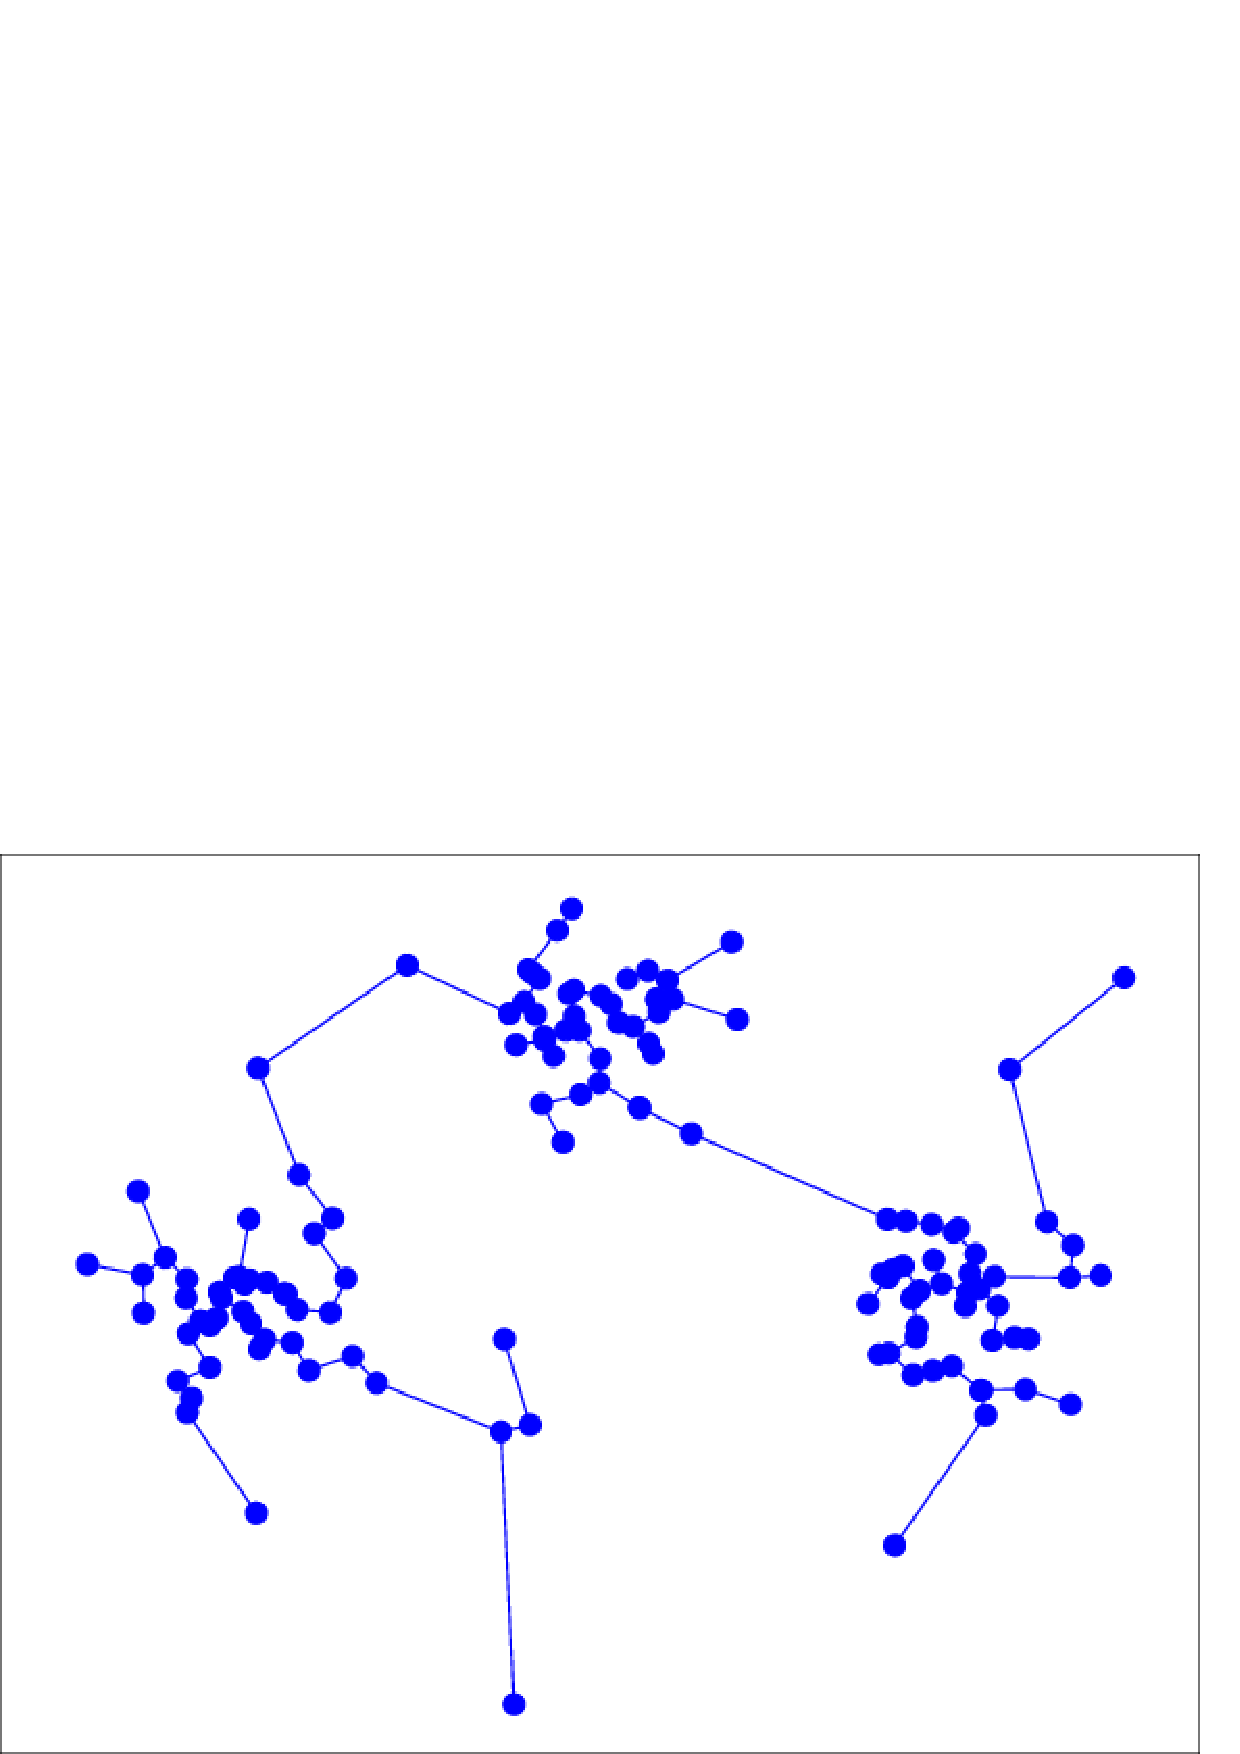
\includegraphics[width=.45\textwidth]{accs_MNIST}
\caption{Runtime comparison of \pystruct and \svmstruct for multi-class
    classification.
}
\label{fig:timings}
\end{figure}


\section{Conclusion}
This paper introduced \pystruct, a modular structured learning and prediction library in Python.
\pystruct is geared towards ease of use, while providing efficient implementations.
\pystruct integrates itself into the scientific Python eco-system, making it easy to use with
existing libraries and applications.
Currently, \pystruct focuses on max-margin and perceptron-based approaches. In the future,
we plan to integrate other paradigms, such as sampling-based learning~\citep{wick2011samplerank},
surrogate objectives (for example pseudo-likelihood), and approaches that allow for a better integration
of inference and learning~\citep{meshi2010learning}.


\chapter{Efficient Exact Learning of Loopy CRFs}



\section{Introduction}
Many classical computer vision applications such as stereo, optical flow, semantic
segmentation and visual grouping can be naturally formulated as image labeling tasks.

Arguably the most popular way to approach such labeling problems is via graphical
models, such as Markov random fields (MRFs) and conditional random fields (CRFs).
MRFs and CRFs provide a principled way of integrating local evidence and
modeling spacial dependencies, which are strong in most image-based tasks.

While in earlier approaches, model parameters were set by hand or using
cross-validation, more recently parameters are often learned using a max-margin
approach.

Most models employ linear energy functions of unary and pairwise interactions,
trained using structural support vector machines (SSVMs). While linear energy
functions lead to learning problems that are convex in the parameters, complex
constraints complicate their optimization. Additionally, inference (or more precisely
loss-augmented prediction) is a crucial part in learning, and can often not be
performed exactly, due to loops in the neighborhood graphs.  % TODO clean up!
Approximations in the inference then lead to approximate learning.

We look at semantic image segmentation, learning a model of pairwise
interactions on the popular MSRC-21 dataset.
The contribution of this work is threefold:
\begin{itemize}
    \item We analyze the simultaneous use of multiple approximate inference
        methods for learning SSVMs using the cutting plane method, relating
        approximate learning to the exact optimum.
    \item We introduce an efficient caching scheme to accelerate cutting plane
        training.
    \item We demonstrate that using a combination of under-generating and exact
        inference methods, we can learn an SSVM exactly in a practical
        application, even in the presence of loopy graphs.
\end{itemize}

While empirically exact learning yields results comparable to those using
approximate inference alone, certification of optimality allows treating
learning as a black-box, allowing the researcher to focus attention on
designing the model for the application at hand.


\section{Related Work}

Max margin learning for structured prediction was introduced by
\citet{taskar2003max}, in the form of maximum-margin Markov models. Later, this
framework was generalized to structural support vector machines by
\citet{tsochantaridis2006large}. Both works assume tractable loss-augmented
inference.

Currently the most widely used method is the one-slack cutting plane formulation
introduced by \citet{joachims2009cutting}.
This work also introduced the caching of constraints,
which serves as a basis for our work. We improve upon their caching scheme, and in
particular consider how it interacts with approximate inference algorithms.

% TODO learning for inference?
Recently, there has been much research in learning structured prediction models
where standard exact inference techniques are not applicable.
The influence of approximate inference on structural support vector machine
learning was first analyzed by  \citet{finley2008training}.
\citet{finley2008training} show convergence results for under-generating and
over-generating inference procedures, meaning methods that find suboptimal, but
feasible solutions, and optimal solutions from a larger (unfeasible) set,
respectively.
\citet{finley2008training} demonstrate that over-generating approaches---in
particular linear programming (LP)---perform best on the considered model.
They also give a bound on the empirical risk for this case.
In contrast, we aim at optimizing the non-relaxed objective directly, yielding
the original, tighter bound.

As using LP relaxations was considered too costly for typical computer vision
approaches, later work employed graph-cuts~\citep{szummer2008learning} or Loopy
Believe Propagation (LBP)~\citep{lucchi2011spatial}. These works use a single
inference algorithm for during the whole learning process, and can not provide any
bounds on the true objective or the empirical risk. In contrast, we combine
different inference methods that are more appropriate for different stages of
learning.

Recently, \citet{meshi2010learning}, \citet{hazan2010primal} and
\citet{komodakis2011efficient} introduced formulations for joint inference and
learning using duality.
In particular, \citet{hazan2010primal} demonstrate the performance of their
model on an image denoising task, where it is possible to learn a large number
of parameters efficiently.
While these approaches show great promise, in particular for pixel-level or
large-scale problems, they perform approximate inference and learning, and do
not relate their results back to the original SSVM objective they approximate.


\begin{algorithm*}[t]
    \caption{Cutting Plane Training of Structural SVMs \label{alg_cutting_plane}}

\begin{algorithmic}[1]
    \Require Training samples $\{ (x^{1}, y^{1}), \dots, (x^{n}, y^{n})\}$, regularization parameter $C$, stopping tolerance $\epsilon$, separation oracle $I$.
    \Ensure Parameters $\theta$, slack $\xi$
    \State $\W \leftarrow \emptyset$
    \Repeat
    \State $(\theta, \xi) \leftarrow \displaystyle \argmin_{\theta, \xi} \frac{||\theta||}{2}^2 + C \xi$\label{restricted}\\
    \begin{equation*}
        \text{s.t. }\forall \hat{\mathbf{y}}=(\hat{y}^1, \dots, \hat{y}^n) \in \W:
        \left \langle \theta, \sum_{i=1}^n [\psi(x^i, y^i) - \psi(x^i,
            \hat{y}^i)] \right \rangle \geq \sum_{i=1}^n \Delta(y^i, \hat{y}^i)
            - \xi
    \end{equation*}
    \For {i=1, \dots, n}
    \State
    $\hat{y}^i \leftarrow I(x^i, y^i, \theta) \approx \displaystyle \argmax_{\hat{y}\in\mathcal{Y}} \sum_{i=1}^n \Delta(y^i, \hat{y}) - \left \langle \theta, \sum_{i=1}^n [\psi(x^i, y^i) - \psi(x^i, \hat{y})] \right \rangle$ \label{get_cutting_plane}
    \EndFor
    \State $\W \leftarrow \W \cup \{ (\hat{y}^1, \dots, \hat{y}^n) \} $
    \State $ \displaystyle \xi' \leftarrow  \sum_{i=1}^n \Delta(y^i, \hat{y}^i) - \left \langle \theta, \sum_{i=1}^n [\psi(x^i, y^i) - \psi(x^i, \hat{y}^i)] \right \rangle$
    \Until $\xi' - \xi < \epsilon$ \label{convergence_check}
\end{algorithmic}
\end{algorithm*}

\section{Efficient Cutting Plane Training of SSVMs}\label{learning}

\subsection{The Cutting Plane Method}\label{cutting_plane}

When learning for structured prediction in the max-margin framework of
\citet{tsochantaridis2006large}, predictions are made as
\[ \argmax_{y \in \mathcal{Y}} f(x, y, \theta),\]
where $x \in \mathcal{X}$ is the input, $y \in \mathcal{Y}$ the prediction, and $\theta$ are the parameters to be learned.
We will assume $y$ to be multivariate, $y=(y_1, \dots, y_k)$ with possibly varying $k$.

The function $f$ measures compatibility of $x$ and $y$ and is a linear function of the parameters $\theta$:
\[f(x, y, \theta) = \langle \theta, \psi(x, y) \rangle.\]
Here $\psi(x, y)$ is a joint feature vector of $x$ and $y$. Specifying a particular SSVM model
amounts to specifying $\psi$.

For a given loss $\Delta$, the parameters $\theta$ are learned by minimizing
the loss-based soft-margin objective
\begin{equation}\label{mainequation}
\min_\theta \frac{1}{2} ||\theta||^2 + C \sum_i  r_i(\theta)
\end{equation}
with regularization parameter $C$, where $r_i$ is a hinge-loss-like upper
bound on the empirical $\Delta$-risk:
\[r_i(x^i, y^i, y) = \left [\max_{y \in \mathcal{Y}} \Delta(y^i, y) + \left<\theta, \psi(x^i, y) - \psi(x^i, y^i) \right > \right]_+ \]

We solve the following reformulation of Equation~\ref{mainequation}, known as one-slack QP formulation:
\begin{align}\label{oneslack}
    \min_{\theta, \xi}\ &\frac{1}{2} ||\theta||^2 + C \xi\\
    \text{s.t. }&\forall \hat{\mathbf{y}}=(\hat{y}^1, \dots, \hat{y}^n) \in \mathcal{Y}^n:\\
        &\left \langle \theta, \sum_{i=1}^n [\psi(x^i, y^i) - \psi(x^i,
            \hat{y}^i)] \right \rangle \geq \sum_{i=1}^n \Delta(y^i, \hat{y}^i)
            - \xi
\end{align}
using the cutting plane method described in
Algorithm~\ref{alg_cutting_plane}~\citep{joachims2009cutting}.

The cutting plane method alternates between solving Equation~\eqref{oneslack}
with a working set $\W$ of constraints, and expanding the working set using the
current $\theta$ by finding $\mathbf{y}$ corresponding to the most violated constraint,
using a separation oracle $I$.
We investigate the construction of $\W$ and the influence of $I$
on learning.

%TODO unstructured!!

Intuitively, the one-slack formulation corresponds to joining all training
samples into a single training example $(\mathbf{x}, \mathbf{y})$ that has no
interactions between variables corresponding to different data points.
Consequently, only a single constraint is added in each iteration of
Algorithm~\ref{alg_cutting_plane}, leading to very small $\W$. We further use
pruning of unused constraints, as suggested by \citet{joachims2009cutting},
resulting in the size of $\W$ being in the order of hundreds for all experiments.

We also use another enhancement of the cutting plane algorithm introduced by
\citet{joachims2009cutting}, the caching oracle. For each training example $(x^i, y^i)$,
we maintain a set $C^i$ of the last $r$ results of loss-augmented inference
(line~\ref{get_cutting_plane} in Algorithm~\ref{alg_cutting_plane}).
For generating a new constraint $(\hat{y}^1, \dotsc, \hat{y}^n)$ we find
\[ 
    \hat{y}^i \leftarrow \argmax_{\hat{y}\in C^i} \sum_{i=1}^n \Delta(y^i, \hat{y}) - \left \langle \theta, \sum_{i=1}^n [\psi(x^i, y^i) - \psi(x^i, \hat{y})] \right \rangle
\]
by enumeration of $C^i$ and continue until line~\ref{convergence_check}.
Only if $\xi' - \xi < \epsilon$, i.e.\ the produced constraint is not violated, we
return to line~\ref{get_cutting_plane} and actually invoke the separation
oracle $I$.

In computer vision applications, or more generally in graph labeling problems,
$\psi$ is often given as a factor graph over $y$, typically using only unary and pairwise functions:
\[ \langle \theta, \psi(x, y) \rangle = \sum_{i=0}^k \langle \theta_u,  \psi_u(x, y_k) \rangle + \sum_{(i, j) \in E} \langle \theta_p, \psi_p(x, y_k, y_l) \rangle, \]
where $E$ a set of pairwise relations. In this form, parameters $\theta_u$ and $\theta_p$ for unary and
pairwise terms are shared across all entries and pairs.
The decomposition of $\psi$ into only unary and pairwise interactions allows
for efficient inference schemes, based on message passing or graph cuts.

There are two groups of inference procedures, as identified in
\citet{finley2008training}: under-generating and over-generating approaches.
An under-generating approach satisfies $I(x^i, y^i, \theta) \in
\mathcal{Y}$, but does not guarantee maximality in line~\ref{get_cutting_plane}
of Algorithm~\ref{alg_cutting_plane}. An over-generating approach on the other
hand, will solve the loss-augmented inference in line~\ref{get_cutting_plane}
exactly, but for a larger set $\hat{\mathcal{Y}} \supset \mathcal{Y}$, meaning
that possibly $I(x^i, y^i, \theta) \notin \mathcal{Y}$.  We will elaborate on
the properties of under-generating and over-generating inference procedures in
Section~\ref{bounds}.


\subsection{Bounding the Objective}\label{bounds}
Even using approximate inference procedures, several statements
about the original exact objective (Equation~\ref{mainequation}) can be
obtained.

Let $o_{\W}(\theta)$ denote objective \eqref{oneslack} with
given parameters $\theta$ restricted to a working set $\W$, as computed in
line~\ref{restricted} of Algorithm~\ref{alg_cutting_plane} and  let
\[
    o^I(\theta) = C\xi' + \frac{||\theta||}{2}^2
\]
when using inference algorithm $I$, i.e. $o^I(\theta)$ is the approximation of the primal
objective given by $I$. To simplify exposure, we will drop the dependency on $\theta$.

Depending on the properties of the inference procedure $I$ used, it is easy to see:
\begin{enumerate}
    \item If all constraints $\hat{y}$ in  $\W$ are feasible, i.e.\ generated
        by an under-generating or exact inference mechanism, then $o_{\W}$ is
        an lower bound on the true optimum $o(\theta^*)$.

    \item If $I$ is an over-generating or exact algorithm, $o^I$ is an upper
        bound on $o(\theta^*)$.
\end{enumerate}

These two observations can be used in a number of ways.
\citet{finley2008training} used 2. to show that learning with an
over-generating approach minimizes an upper bound on the empirical risk.

We can also use these observations to judge the suboptimality of a given parameter $\theta$,
i.e.\ see how far the current objective is from the true optimum.
Learning with any under-generating approach, we can use 1. to maintain a lower bound
on the objective. At any point during learning, in particular if no more constraints
can be found, we can then use 2., to also find an upper bound.
This way, we can empirically bound the estimation error, using only approximate
inference.
We will now describe how we can further use 1. to both speed up and improve learning.


\subsection{Combining Inference Procedures}\label{combining}
The cutting plane method described in Section~\ref{cutting_plane} relies only
on some separation oracle $I$ that produces violated constraints.

Using any under-generating oracle $I$, learning can proceed as long as a
constraint is found that is violated by more than the stopping tolerance
$\epsilon$.  Which constraint is used next has an impact on the speed of
convergence, but not on correctness. Therefore, as long as an under-generating
method does generate constraints, optimization makes progress on the objective.

Instead of choosing a single oracle, we propose to use a succession of
algorithms, moving from fast methods to more exact methods as training
proceeds. This strategy not only accelerates training, it even makes it
possible to train with exact inference methods, which is infeasible otherwise.

In particular, we employ three strategies for producing constraints,
moving from one to the next if no more constraints can be found:
\begin{enumerate*}
    \item Produce a constraint using previous, cached inference results.
    \item Use a fast under-generating algorithm.
    \item Use exact inference.
\end{enumerate*}

While using more different oracles is certainly possible, we found
that using just these three methods performed very well in practice.  This
combination allows us to make fast progress initially and guarantee optimality
in the end.
Notably, it is not necessary for an algorithm used as 3) to always produce
exact results. For guaranteeing optimality of the model, it is sufficient that
we obtain a certificate of optimality when learning stops.

\subsection{Dynamic Constraint Selection}\label{caching}
Combining inference algorithm as described in Section~\ref{combining}
accelerates calls to the separation oracle by using faster, less accurate
methods. On the down-side, this can lead to the inclusion of many constraints
that make little progress in the overall optimization, resulting in much more
iterations of the cutting plane algorithm. We found this particularly problematic
with constraints produced by the cached oracle.

We can overcome this problem by defining a more elaborate schedule to switch
between oracles, instead of switching only if no violated constraint can be
found any more. Our proposed schedule is based on the intuition that we only
trust a separation oracle as long as the current primal objective did not move
far from the primal objective as computed with the stronger inference
procedure.

%More precisely, let $o_{\W}(\theta)$ denote objective \eqref{oneslack} with
%given parameters $\theta$ restricted to a working set $\W$, as computed in
%line~\ref{restricted} of Algorithm~\ref{alg_cutting_plane} and  let
%\[
    %o^I(\theta) = C\xi' + \frac{||\theta||}{2}^2
    %\]
%when using inference algorithm $I$, i.e. $o^I(\theta)$ is the approximation of the primal
%objective given by $I$. To simplify exposure, we will drop the dependency on $\theta$.
In the following, we will use the notation of Section~\ref{bounds} and indicate
the choices of oracle $I$ with $Q$ for a chosen inference algorithm and $C$ for
using cached constraints.

To determine whether to produce inference results from the cache or to run the inference algorithm,
we solve the QP once with a constraint from the cache. If the resulting $o^C$ verifies
\begin{equation}\label{cache_test}
    o^C - o^Q < \frac{1}{2} (o^Q - o_{\W})
\end{equation}
we continue using the caching oracle. Otherwise we run the inference algorithm again.
For testing \eqref{cache_test}, the last known value of $o^Q$ is used, as recomputing it would defy
the purpose of the cache.

It is easy to see that our heuristic runs inference only $O(\log(o^Q -
o_{\W}))$ times more often than the strategy from \citet{joachims2009cutting} in the
worst case.



\section{Experiments}
\subsection{Inference Algorithms}
As a fast under-generating inference algorithm, we used $\alpha$-expansion
moves based on non-submodular graph-cuts using Quadratid Pseudo-Boolean
Optimization (QPBO)~\citep{rother2007optimizing}.  This move-making strategy
can be seen as a simple instantiation of the more general framework of fusion
moves, as introduced by \citet{lempitsky2010fusion}

For exact inference, we use the recently developed Alternating Direction Dual
Decomposition (AD$^3$) method of \citet{martins2011augmented}. AD$^3$ produces
a solution to the linear programming relaxation, which we use as the basis for
branch-and-bound.

\begin{table}
    \begin{center}
    \begin{tabular}{lcc}
        \toprule
                    & Average & Global \\
        \cmidrule{1-3}
    Unary terms only & 77.7& 83.2 \\
    Pairwise model (move making)& 79.6&84.6\\
    Pairwise model (exact)& 79.0 & 84.3\\
        \cmidrule{1-3}
    \citet{ladicky2009associative} & 75.8& 85.0\\
    \citet{gonfaus2010harmony} & 77&  75\\
    \citet{lucchi2013learning} & 78.9& 83.7\\
    \bottomrule
    \end{tabular}
    \end{center}
    \caption{Accuracies on the MSRC-21 Dataset.  We compare a baseline model,
    our exact and approximately learned models and state-of-the-art
    approaches.\label{msrcacc}}
    
\end{table}


%\subsection{Multi-Label Classification}
%TODO

%\subsection{Snake}
%TODO

\subsection{Image Segmentation}
We choose superpixel-based semantic image segmentation as sample application
for this work.  CRF based models have a history of success in this application,
with much current work investigating models and
learning~\citep{gonfaus2010harmony, lucchi2013learning, ladicky2009associative,
kohli2009robust, krahenbuhl2012efficient}.  We use the MSRC-21 and Pascal VOC 20120 datasets, two
widely used benchmark in the field.

We use the same model and pairwise features for the two datasets.
Each image is represented as a neighborhood graph of superpixels.
For each image, we extract approximately 100 superpixels using 
the SLIC algorithm~\citep{achanta2012slic}.

We introduce pairwise interactions between neighboring superpixels, as is
standard in the literature. Pairwise potentials are founded on two
image-based features: color contrast between superpixels, and relative location
(coded as angle), in addition to a bias term.

We set the stopping criterion $\epsilon=10^{-4}$, though using only
the under-generating method, training always stopped prematurely as no violated
constraints could be found any more.

\subsection{Caching}
First, we compare our caching scheme, as described in Section~\ref{combining}, with the
scheme of \citet{joachims2009cutting}, which produces constrains from the cache
as long as possible, and with not using caching of constraints at all.  For this experiment,
we only use the under-generating move-making inference on the MSRC-21 dataset. Times until convergence
are 397s for our heuristic, 1453s for the heuristic of
\citet{joachims2009cutting}, and 2661s for using no cache, with all strategies
reaching essentially the same objective.

Figure~\ref{caching} shows a visual comparison that highlights the differences
between the methods. Note that neither $o^Q$ nor $o^C$ provide valid upper bounds on the objective,
which is particularly visible for $o^C$ using the method of \cite{joachims2009cutting}.
Using no cache leads to a relatively smooth, but slow convergence, as inference is run often.
Using the method of \citet{joachims2009cutting}, each run of the separation oracle is followed by
quick progress of the dual objective $o_\W$, which flattens out quickly. Much time is then spent adding
constraints that do not improve the dual solution.
Our heuristic instead probes the cache, and only proceeds using cached constraints if the resulting
$o^C$ is not to far from $o^Q$.

\begin{figure*}
\centering
\includegraphics[width=.7\linewidth]{caching}
\caption{%
Training time comparison using different caching heuristics.
Large dots correspond to $o^Q$, small dots correspond to $o^C$,
and the line shows $o_\W$. See the text for details.\label{caching}}
\end{figure*}
% much simpler model?


\subsubsection{MSRC-21 Dataset}
For the MSRC-21 Dataset, we use unary potentials based on bag-of-words of SIFT
features and color features.  Following \citet{lucchi2011spatial} and
\citet{fulkerson2009class}, we augment the description of each superpixel by a
bag-of-word descriptor of the whole image. To obtain the unary potentials for
our CRF model, we train a linear SVM using the additive $\chi^2$ transform
introduced by \citet{vedaldi2010efficient}. Additionally, we use the unary
potentials provided by \citet{krahenbuhl2012efficient}, which are based on
TextonBoost~\citep{shotton2006textonboost}. This leads to $42 = 2 \cdot 21$
unary features for each node.

The resulting model has around 100 output variables per image, each taking one of 21
labels. The model is trained on 335 images from the standard training and
validation split.

\begin{table}
    \begin{center}
    \begin{tabular}{lc}
        \toprule
                    & Jaccard \\
        \cmidrule{1-2}
    Unary terms only &  27.5 \\
    Pairwise model (move making)& 30.2\\
    Pairwise model (exact) & 30.4\\
        \cmidrule{1-2}
    \citet{dann2012pottics} & 27.4\\
    \citet{krahenbuhl2012efficient} & 30.2\\
    \citet{krahenbuhlparameter} & 30.8\\
    \bottomrule
    \end{tabular}
    \end{center}
    \caption{Accuracies on the Pascal VOC Dataset. We compare our approach
    against approaches using the same unary potentials.\label{pascalacc}}
    
\end{table}


\subsubsection{Pascal VOC 2010}
For the Pascal VOC 2010 dataset, we follow the procedure from \citet{krahenbuhl2012efficient}
in using the official ``validation'' set as our evaluation set, and splitting the training set again.
We use the unary potentials provided by the same work, and compare only against methods
using the same setup and potentials, \citet{krahenbuhlparameter} and \citet{dann2012pottics}.
Note that state-of-the-art approaches, some not build on the CRF framework, obtain
around 40\% Jaccard score (also call VOC score), notably \cite{xia2012segmentation}, who 
evaluate on the Pascal VOC 2010 ``test'' set.


\begin{table}
    \begin{center}
    \begin{tabular}{lcc}
    \toprule
                    & Move-making & Exact \\
    \cmidrule{1-3}
    Dual Objective $o_\W$ & 65.10 & 67.66  \\
    Estimated Objective $o^I$ &  67.62& 67.66\\
    True Primal Objective $o^E$& 69.92& 67.66\\
    \bottomrule
    \end{tabular}
    \end{center}
    \caption{Objective function values on the MSRC-21 Dataset}
    \label{msrc_objective}
\end{table}

\subsubsection{Results}
We compare classification results using different inference schemes in
with results from the literature. As a sanity check, we
also provide results without pairwise interactions.

Results on the MSRC-21 dataset are shown in Table~\ref{msrcacc}.
We find that our model is on par with state-of-the-art approaches, implying
that our model is realistic for this task. In particular, our results are comparable to those of
\citet{lucchi2013learning}, who use a stochastic subgradient method with working sets.
Their best model takes 583s for training, while training our model exactly takes 1814s.
We find it remarkable that it is possible to guarantee optimality in time of
the same order of magnitude that a stochastic subgradient procedure with
approximate inference takes. Using exact learning and inference does not increase accuracy
on this dataset.
Learning the structured prediction model using move-making inference alone
takes 4 minutes, while guaranteeing optimality up to  $\epsilon=10^{-4}$
takes only 18 minutes.

Results on the Pascal-VOC dataset are shown in Table~\ref{pascalacc}.
We compare against several approaches using the same unary potentials.
For completeness, we also list state-of-the-art approaches not based on CRF models.
Notably, out model matches or exceeds the performance of the much more involved approaches of
\citet{krahenbuhl2012efficient} and \citet{dann2012pottics} which use the same
unary potentials.
Using exact learning and inference slightly increased performance on this dataset.
Learning took 25 minutes using move-making alone and 100 minutes to guarantee optimality
up to $\epsilon=10^{-4}$.
A visual comparison of selected cases is shown in Figure~\ref{visual}.


The objective function values using only the under-generating move-making and
the exact inference are detailed in Table~\ref{msrc_objective} and Table~\ref{pascal_objective}.
We see that a significant gap between the cutting plane objective and the primal objective
remains when using only under-generating inference.
Additionally, the estimated primal objective $o^I$ using under-generating inference is
too optimistic, as can be expected. This underlines the fact that
under-generating approaches can not be used to upper-bound the primal
objective.

\begin{table}
    \begin{center}
    \begin{tabular}{lcc}
    \toprule
                    & Move-making & Exact \\
    \cmidrule{1-3}
    Dual Objective $o_\W$ &92.06& 92.24\\
    Estimated Objective $o^I$ & 92.07 &92.24\\
    True Primal Objective $o^E$&92.35& 92.24  \\
    \bottomrule
    \end{tabular}
    \end{center}
    \caption{Objective function values on the Pascal Dataset.}
    \label{pascal_objective}
\end{table}


\subsection{Implementation Details}
We implemented the cutting plane Algorithm~\ref{alg_cutting_plane} and our pairwise
model in Python.
Our cutting plane solver for Equation~\eqref{mainequation} uses
\texttt{cvxopt}~\citep{dahl2006cvxopt} for solving the QP in the inner loop. Code for
our structured prediction framework will be released under an open source
license upon acceptance.

We used the SLIC implementation provided by \citet{achanta2012slic} to extract superpixels and
the SIFT implementation in the \texttt{vlfeat} package~\citep{vedaldi08vlfeat}.
For clustering visual words, piecewise training of unary potentials and the
approximation to the $\chi^2$-kernel, we made use of the \texttt{scikit-learn}
machine learning package~\citep{pedregosa2011scikit}.
The move-making algorithm using QPBO is implemented with the help of the QPBO-I
method provided by \citet{rother2007optimizing}.
We use the excellent implementation of AD$^3$ provided by the authors of
\citet{martins2011augmented}. 

Thanks to using these high-quality implementations, running the whole pipeline
for the pairwise model takes less than an hour on a 12 core CPU\@. Solving the
QP is done in a single thread, while inference is parallelized over all cores.
 
\section{Discussion}
In this work we demonstrated that it is possible to learn state-of-the-art CRF models
exactly using structural support vector machines, despite the model containing many loops.
The key to efficient learning is the combination of different inference mechanisms and
a novel caching scheme for the one-slack cutting plane method, in combination
with state-of-the-art inference methods.

We show that guaranteeing exact results is feasible in a practical setting, and
hope that this result provides a new perspective onto learning loopy models for
computer vision applications.

Even though exact learning does not necessarily lead to a large improvement in
accuracy, it frees the practitioner from worrying about optimization and
approximation issues, leaving more room for improving the model, instead of the
optimization.

While our model is trained on a relatively small dataset, we expect that scaling to
datasets of several thousand images, such as Pascal VOC, is unproblematic.
The time for a single iteration of the cutting plane solver will only grow
linearly for the inference. The cost of solving the QP is actually independent
of the number of samples, as only a single constraint will be added in each
iteration.

We do not expect learning of pixel-level models, which typically have tens or
hundreds of thousands of variables, to be efficient using exact inference. However we
believe our results will carry over to other super-pixel based approaches.
Using other over-generating techniques, such as duality-based message passing
algorithms, it might be possible to obtain meaningful bounds on the true
objective, even in the pixel-level domain.

\begin{figure*}
\centering
\includegraphics[width=\linewidth]{figure}
\caption{%
    Visual comparison of the result of exact and approximate learning on
    selected images from the test set.  From left to right: the input image,
    prediction using approximate learning, prediction using exact learning, and
    ground truth.
\label{visual}}
\end{figure*}



\chapter{Hierarchical Latent Variable Models for Semantic Segmentation}

\bibliography{main}
\end{document}
